%Replace Strings:
%PROJECT.TITLE
%TODO.CHANGE
%PROJECT.ABSTRACT.KEYWORDS

\documentclass[12pt, a4paper, oneside]{article}

\usepackage[utf8]{inputenc}
\usepackage[bindingoffset=1.57cm, left=2.54cm, right=2.54cm, top=2.54cm, bottom=2.54cm]{geometry}
\usepackage{mathptmx}
\usepackage{fancyhdr}
\usepackage{lipsum}
\usepackage{secdot}
\usepackage{lastpage}
\usepackage{cite}
\usepackage{tabularx}
\usepackage{booktabs}



\usepackage{graphicx}
	\graphicspath{ {images/} }

\usepackage{tocloft}
\usepackage[table,xcdraw]{xcolor}

\usepackage{floatrow}
\floatsetup[table]{capposition=top}

\linespread{1.2}
\pagestyle{fancy}
\fancyhf{} % sets both header and footer to nothing
\renewcommand{\headrulewidth}{0pt}
\rhead{ \textit{Treasure Nepal: Discover Places, Collect Treasures}}
\cfoot{\thepage}

\setlength{\parindent}{0pt}
\setlength{\parskip}{12pt}

%\frontmatter

\begin{document}

\pagenumbering{roman}

\addcontentsline{toc}{section}{Acknowledgement}
\large
\begin{center}
	\textbf{ACKNOWLEDGEMENT}
\end{center}

\normalsize
\vspace{40px}
\lipsum[2]

\break

\addcontentsline{toc}{section}{Abstract}
\large
\begin{center}
	\textbf{ABSTRACT}
\end{center}

\normalsize
As we are at the brim of the Visit Nepal year 2020, the decentralization of tourism in Nepal has become absolutely necessary. Almost ninety percent of the tourists arriving Nepal visit the most popular destinations like Kathmandu, Pokhara, Chitwan and Everest, whereas the remote places like Rara Lake and Phoksundo National Park have not seen satisfactory inflow of tourists despite them being rich in natural beauty and tourism potentiality. There are still a lot of tourist destinations in Nepal that need the attention of the tourists.

Treasure Nepal is a treasure hunt application where the users travel to different places in order to collect treasures and increase their scores. The app has an integrated map that navigate the users to various tourist destinations in Nepal. The project aims to take the attention of tourists and visitors towards various tourists destinations in Nepal. The tourists need to physically reach to a place in order to collect treasures. The tourists who collect treasures at places that are remote and left behind will get higher scores than the ones who visit common popular destinations. The users can also share their scores and leaderboard status to social media. On the long run, the project sets its objective to take the tourism of Nepal to a new level.

This report has been prepared to demonstrate the progress the team has made after the acceptance of project proposal. It also includes major milestones that will be met in future and estimated date for deployment.

\textbf{Keywords}: Visit Nepal 2020, Treasure hunt, Tourism\\

\break

\large
\addcontentsline{toc}{section}{Table of Contents}
\begin{center}
	\textbf{TABLE OF CONTENTS}
\end{center}


\normalsize
\setlength{\cftbeforetoctitleskip}{0pt}
\renewcommand{\contentsname}{}
\tableofcontents

\break

\large
\addcontentsline{toc}{section}{List of Figures}
\begin{center}
	\textbf{LIST OF FIGURES}
\end{center}
\renewcommand{\listfigurename}{}

\listoffigures

\break

\large
\addcontentsline{toc}{section}{List of Tables}
\begin{center}
	\textbf{LIST OF TABLES}
\end{center}
\renewcommand{\listtablename}{}

\listoftables

\break

%\mainmatter
\cfoot{\textbf{\thepage} /  \pageref{LastPage}}

\pagenumbering{arabic}
\section{Introduction} 
Treasure Nepal is a mobile application for a treasure hunt game proposed to be tailored for tourists visiting Nepal. With the view of encouraging tourists to visit remote and unexplored part of the country, the application aims to increase the traffic of tourist in such locations as well as promote their tourism. This document looks forward to providing detailed information about the project, the tasks that have been done so far, and the tasks that are remaining.

Tourism has a great potential to contribute to the Gross Domestic Product (GDP) of Nepal, but having observations at the statistics, the ratio of contribution of tourism to GDP is not satisfactory. According to Nepal Rastra Bank, the total contribution of the foreign exchange from tourism to the total Gross Domestic Product (GDP) of Nepal was 2.2\% in the year 2017/18. \cite{tourismstats}.

The Government of Nepal has taken efforts to celebrate the year 2020 officially as the Visit Nepal Year 2020. At the brim of year 2020, the authors have proposed to build a treasure hunt application specially tailored for the tourists to get their attention to unexplored and remote tourism destinations of Nepal. 

There are a few applications somehow similar to the proposed application but none of them are built for tourism purposes. Rather, they are developed only for entertainment purposes. In this context, this application will distinguish itself as unique and first of the kind product in the market.

Tourism in Nepal is largely centralized to a few popular destinations. The places like Kathmandu, Pokhara, Chitwan, Annapurna area and Everest area are largely flocked by tourists while destinations like Rara Lake, Shey Phoksundo National Park or Khaptad National park struggle to get satisfactory inflow of traffic.

\subsection{Problem Statement}
The decentralisation of tourism has largely underestimated the potential and beauty of many travel destinations, specially in remote areas. As a result, these places have very low traffic of tourists. In addition, as majority of people in such places rely solely on tourism industry for their livelihood, this problem has pushed those communities even further down below the poverty line.

\subsection{Project Objectives}
The project has put forward the following objectives:

\begin{itemize}
	\item To decentralize the tourism industry and encourage uniform flow of tourists at various destinations across Nepal.
	\item To promote and encourage the tourism in remote and novel destinations which otherwise are not popular or have low inflow of tourists.
	\item To explore business and economic opportunities generated by the project if taken to the production level.
\end{itemize}

\subsection{Significance of the Study}
The project is significant owing to the fact that we are near the Visit Nepal Year 2020, and it will certainly be fruitful in achieving the objectives set by the Government of Nepal in the year 2020. Since the idea behind is one of the first of its kind, it is expected that the project will reach to a significant majority of tourists that visit Nepal in 2020.

\subsection{Scope and Limitations}
In the beginning phase, the treasure hunt concept of the app will be implemented and other features are proposed to be added later gradually if possible. Such possible extensions could be addition of forex plugins, itinerary maps, guides, etc. The users will be able to collect coins from collecting the treasures, and their collection will be put in the leaderboards based on the user's local location as well as country-wise and globally. The application will have an integrated map, which enlists the tourist destinations in the locality of tourist's current location. The application will also be connected to third party social networking platforms like Facebook, Twitter, etc. so that the users can share their collection and score. 

The scores of the treasures will be calculated based on the factors like the difficulty to reach the destination, its novelty, potentiality to attract new tourists and other similar criteria. The users will receive more amount of score when visiting rural and novel places than visiting urban and frequently visited places.

The following are the limitations of the project that are realized:
\begin{itemize}
 	\item The application will be built on Android and iOS platform, but not for other mobile operating systems like Blackberry and Windows.
	\item QR code scanning will be the method of collection of treasures and no other validation architecture will be used except for the check of location when the user scans the QR.
 \end{itemize}

\break
\section{Literature Review}
This section consists description of the literature study performed during the development of this proposal.

\subsection{Visit Nepal 2020}
The Visit Nepal 2020 project was officially introduced by Nepal Tourism Board (NTB) in 2015. The project aims to bring two million tourists in Nepal during the year 2020 \cite{visitnepal}. The slogan of Visit Nepal 2020 has been translated to more than ten different languages. The board also is planning to train ten thousand people to provide quality service to the tourists. 

\subsection{Attractions in Nepal}
The major itineraries of the tourists visiting Nepal include mountaineering, trekking, religious pilgrimages and holiday spending. The northern part of Nepal has the mountain range with highest elevation in the world, called as the Himalayas \cite{himalayas}. These mountains serve as a destination for the tourists seeking mountaineering as welll as trekking. The famous trekking destinations in Nepal are Everest Base Camp, Annapurna Circuit and Langtang Trekking Route \cite{trekkingroutes}. Other attractions include various lakes, the famous of which are Tilicho Lake, Rara Lake, Phewa Lake and Gosaikunda.

Nepal is also rich in biodiversity. Currently there are 12 national parks, 1 wildlife reserve, 6 conservation areas, 1 hunting reserve and 10 Ramsar sites as the protected areas of Nepal \cite{protectedareas}. Among them, Chitawan National Park is the most popular one. A lot of tourists visit these areas for the purpose of jungle safari and animal sports.

Nepal is rich in cultural diversity too. A large portion of the tourist inflow in Nepal occurs for religious and pilgrimage purposes. In recent years, the various communities have incorporated home stay programmes to host tourists in their home and offer their cultural courtesy, which has sent setup good environment for the cultural tourism in Nepal. The festivals like Dashain, Lhosar, Chhath, Gai Jatra, Buddha Jayanti, etc. are some of the most popular festivals of Nepal.

\subsection{Existing Similar Appilcations}
There are several treasure hunt applications available in the application stores developed for entertainment purposes. Some of them are GooseChase, Locandy, Huntzz, Scavify and Geocaching \cite{similarapps}. This application distinguishes itself from these applications due to its focus on the tourism industry. The available applications are developed only for entertainment purposes. Also, the users themselves have to set treasures and spots and enter them into the application to create a challenge and then challenge someone else to find and collect them. In contrast, the users of the proposed application are already provided with the treasures and they don't actively take participation in creating one.

\subsection{Challenges}
One of the major challenges realized is the validation of the collection of treasures by the users. If only QR code is used for validating that a tourist has in fact reached a destination, there is a high chance that the QR codes get shared among people and people will remotely validate themselves having gone to a place and collected a treasure just by scanning the photo of the QR from a remote location. A countermeasure that can be used is to add actual location data from the user's phone's GPS sensor as an additional parameter for validation. A treasure is only considered to be collected if a user scans the QR from within a specific distance from the actual treasure location.

GPS spoofing is one of the major challenges for any system that has used GPS for the validation. GPS spoofing is the process of modifying a GPS receiver unit so that it broadcasts incorrect GPS signal. Some countermeasures to tackle GPS spoofing are monitoring absolute as well as relative GPS signal strength; checking time intervals and performing comparison; and performing sanity checks \cite{gpsspoofmeasures}.

\subsection{Cross Platform App Development}
Android and iOS are two major mobile development platforms in the market today. Any application that is developed targeting both of these platforms is known as a cross platform application. In today's market, the businesses have opted to allow all of their users use their services through all of the technological platforms available to the client. For example, the same services can be used by a web based portal, an Android mobile phone, an iPhone, iPad, or even a desktop computer software.

When cross platform applications are needed to be developed, the two most popular frameworks are Flutter and React Native. React Native is relatively older technology first released in 2013. Currently it is managed by Facebook. Flutter, a new technology, is the similar framework from Google. React Native uses JavaScript as its language while Flutter uses Dart. React Native being older has relatively wider support and user base than flutter. Flutter is rapidly increasing its user base too. The choice between one of them depends upon the programmer's preferences and choices.

\subsection{REST API}
REST stands for Representational State Transfer. It is a software architecture that defines a set of constraints for creation of web services and APIs. The web services that abide by these constraints are called RESTful. The web services are the programs that are run in the server that respond to various HTTP requests like GET, PUT, POST, DELETE, etc. and send response to the client of those services.

API stands for Application Programming Interface. It is a kind of abstract interface or a communication protocol between a client and a server to ease client-server communication. An API can be Web based, OS based, or for a database management system. Web based APIs are those which provide the interface between the client and the database. Each time a client sends a request to the API server, it breaks it down to different database operations and then read/write data to the database. The API server also sends back the data it receives from the database in formats like XML(Extensive Markup Language) or JSON(JavaScript Object Notation).

\break
\section{Methodology}
This section describes the methodology that have been followed during the development of the project.

\subsection{Proposed Software Development Life Cycle}
The project has been developed as per the waterfall model of software development life cycle as depicted in Figure \ref{fig:sdlc}. The reason for choosing this model is the lack of sufficient time duration for agile and iterative methods, as well as very low chances of the changes of requirements in the process of development. 

\begin{figure}[h]
	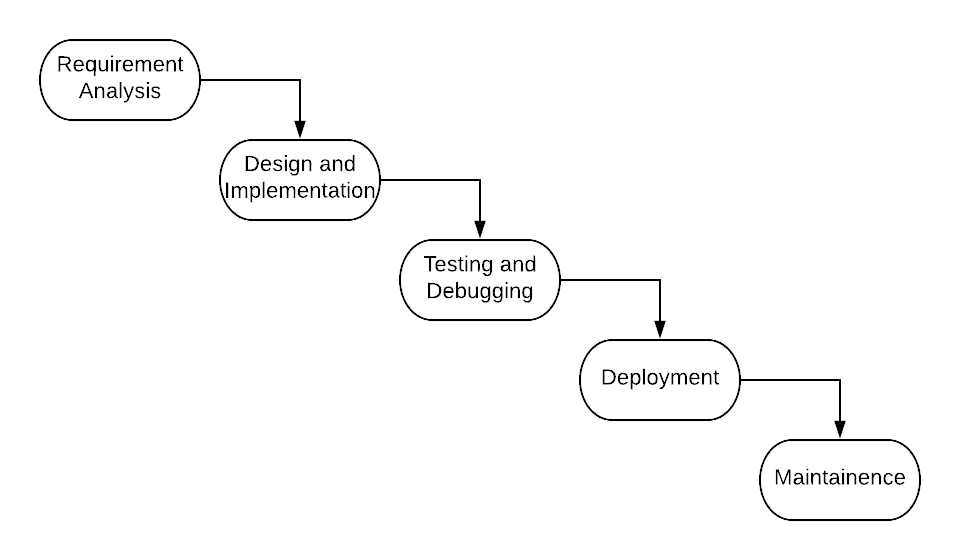
\includegraphics[width=\linewidth]{sdlc}
	\centering
	\caption{Proposed software development life cycle}
	\label{fig:sdlc}
\end{figure}

The life cycle begins when the team collects and evaluates the requirements that will be expected from the application. The design and implementation phase will be to design and build both API services and client applications. By the end of this phase, a minimal viable product (MVP) will already have been constructed. In the testing and debugging phases, the quality control methods will be applied to both API and application. Finally, the application will be deployed to the Amazon Web Services at the end of the deployment phase. However, there might be slight modifications in the original waterfall model where the design and implementation may be changed slightly after the testing phase if seen reasonable.

\subsection{Technical Architecture}
The application has been built upon the client-server web architecture, as illustrated in Figure \ref{fig:arch}.

\begin{figure}[h]
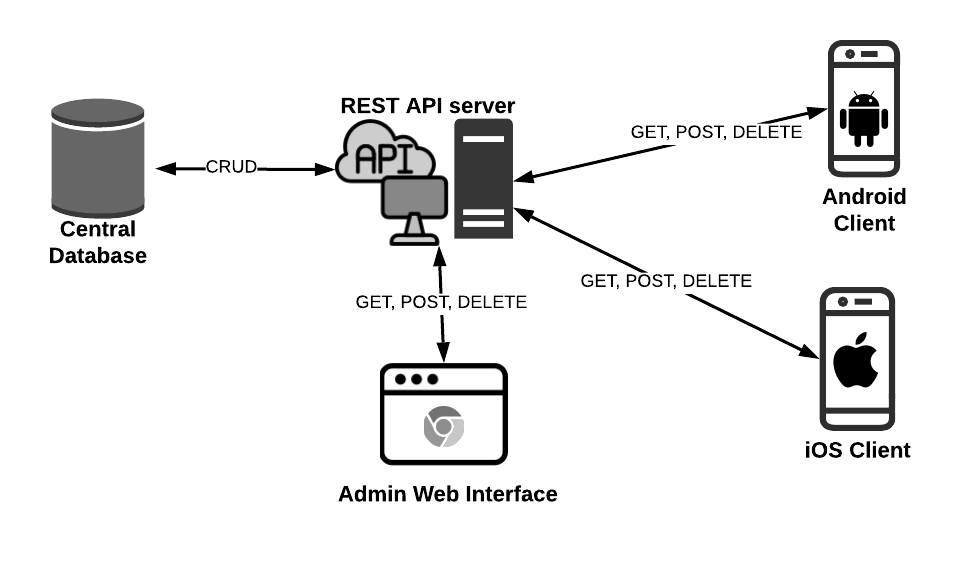
\includegraphics[width=\linewidth]{architecture}
\centering
\caption{Technical architecture of the application}
\label{fig:arch}
\end{figure}

At the heart of the architecture lies the RESTful web service which communicates directly with the central database where all the data is stored. The mobile applications as well as the admin web interface do not access the database directly, but via the API service. The clients send HTTP requests like GET, POST and DELETE, while the API service processes those requests and return the data in JSON format.

\subsection{Technologies Used}
Table \ref{table:tech} consists of the major technologies that are proposed to be used during development and deployment of the application. They are briefly described in the subsections that follow.

\renewcommand{\arraystretch}{1.5}
\begin{table}[]
\begin{tabular}{|l|l|}
\hline
\rowcolor[HTML]{C0C0C0} 
\textbf{Subject}    & \textbf{Proposed Technology} \\ \hline
Backend Database            & MySQL                        \\ \hline
REST API Service    & Django REST Framework        \\ \hline
Android Client  & React Native                 \\ \hline
Deployment Platform & Amazon Web Services (AWS)    \\ \hline
Documentation & LaTeX \\ \hline
\end{tabular}
\caption{Technologies proposed to be used}
\label{table:tech}
\end{table}

\subsubsection{MySQL}
MySQL is one of the most widely used relational database management system (RDBMS). The major reason for us to choose this database is that it is completely open source. Some of the established tech corporates like Facebook, Twitter, Youtube etc. use MySQL. It also has very good user base and the usage is easier thanks to comprehensive documentation and support.

\subsubsection{Django REST Framework}
Django REST framework is an open source framework for building Web APIs. The framework provides features like authentication, tokenization, session handling, serialization, etc. for users to build API in short amount of time. The language used is Python.

\subsubsection{React Native}
React Native is an open source framework for building mobile applications using Javascript language. In addition to the usage of widely used language like Javascript, it also has cross platform support so that both Android and iOS applications can be built using same code base.

\subsubsection{Amazon Web Services (AWS)}
Amazon Web Services (AWS) is a common cloud platform that provides cloud based services to individuals, governments and corporates on the pay-as-you basis. It is a subsidiary of Amazon Inc.

\subsubsection{LaTeX}
LaTeX is widely used documentation preparation system for preparation of scientific documents, books and technical papers. It uses plain text for formatting unlike other document creation systems. The source code is compiled by a compeller to generate the printable/viewable document.

\pagebreak
\section{Tasks Done so Far}
This section enlists the major breakthroughs achieved during the project. Among the total works proposed in the proposal, about two thirds of the progress have already been achieved and the foundation for the next one third have also been laid out.

\subsection{Requirement Analysis}
The requirement analysis of the product to be developed was done before everything else during the project. During this phase, our team worked together to find out what features were expected of the product to be developed. It was also helpful to filter what is important and what is not important features to be added in the application. The requirements were widely classified into two categories: functional and non functional requirements. Functional requirements are those requirements which define a system or a component by the functions it should perform. Non functional requirements are those which describe quality attributes in a system.

The most widely used tool during the requirement analysis phase in our project was the use case descriptions and diagrams. The project team members first described the actions a user would perform on the system during a particular scenario, and then it was converted to diagrammatic form. 


\begin{table}[h!]
\centering
\begin{tabularx}{\linewidth}{|X|} 
\hline
\textbf{Use Case:  Use Application}\\ 
\hline
When the user first installs the app, she should be able to sign up for a new account. For so, the user can either use email address or use Facebook and Google for authentication. Once the user registers her account, she will enter her credentials and login to the application. The user now can see her points (which will be 0 at the start), and all the treasures around her location. She will also be able to get the information about the particular treasure. To collect the treasure, the user will physically have to reach the location where the treasure is installed. When the user checks in at the treasure location, she will be awarded with the points associated with that treasure. The user will be able to see different rewards and offers that she is eligible to collect. She will be able to collect any of the permitted rewards by scanning the QR provided by the offerer. The user can challenge other friends as well as share the app in the social media.\\
\hline
\end{tabularx}
\end{table}

\begin{figure}[h!]
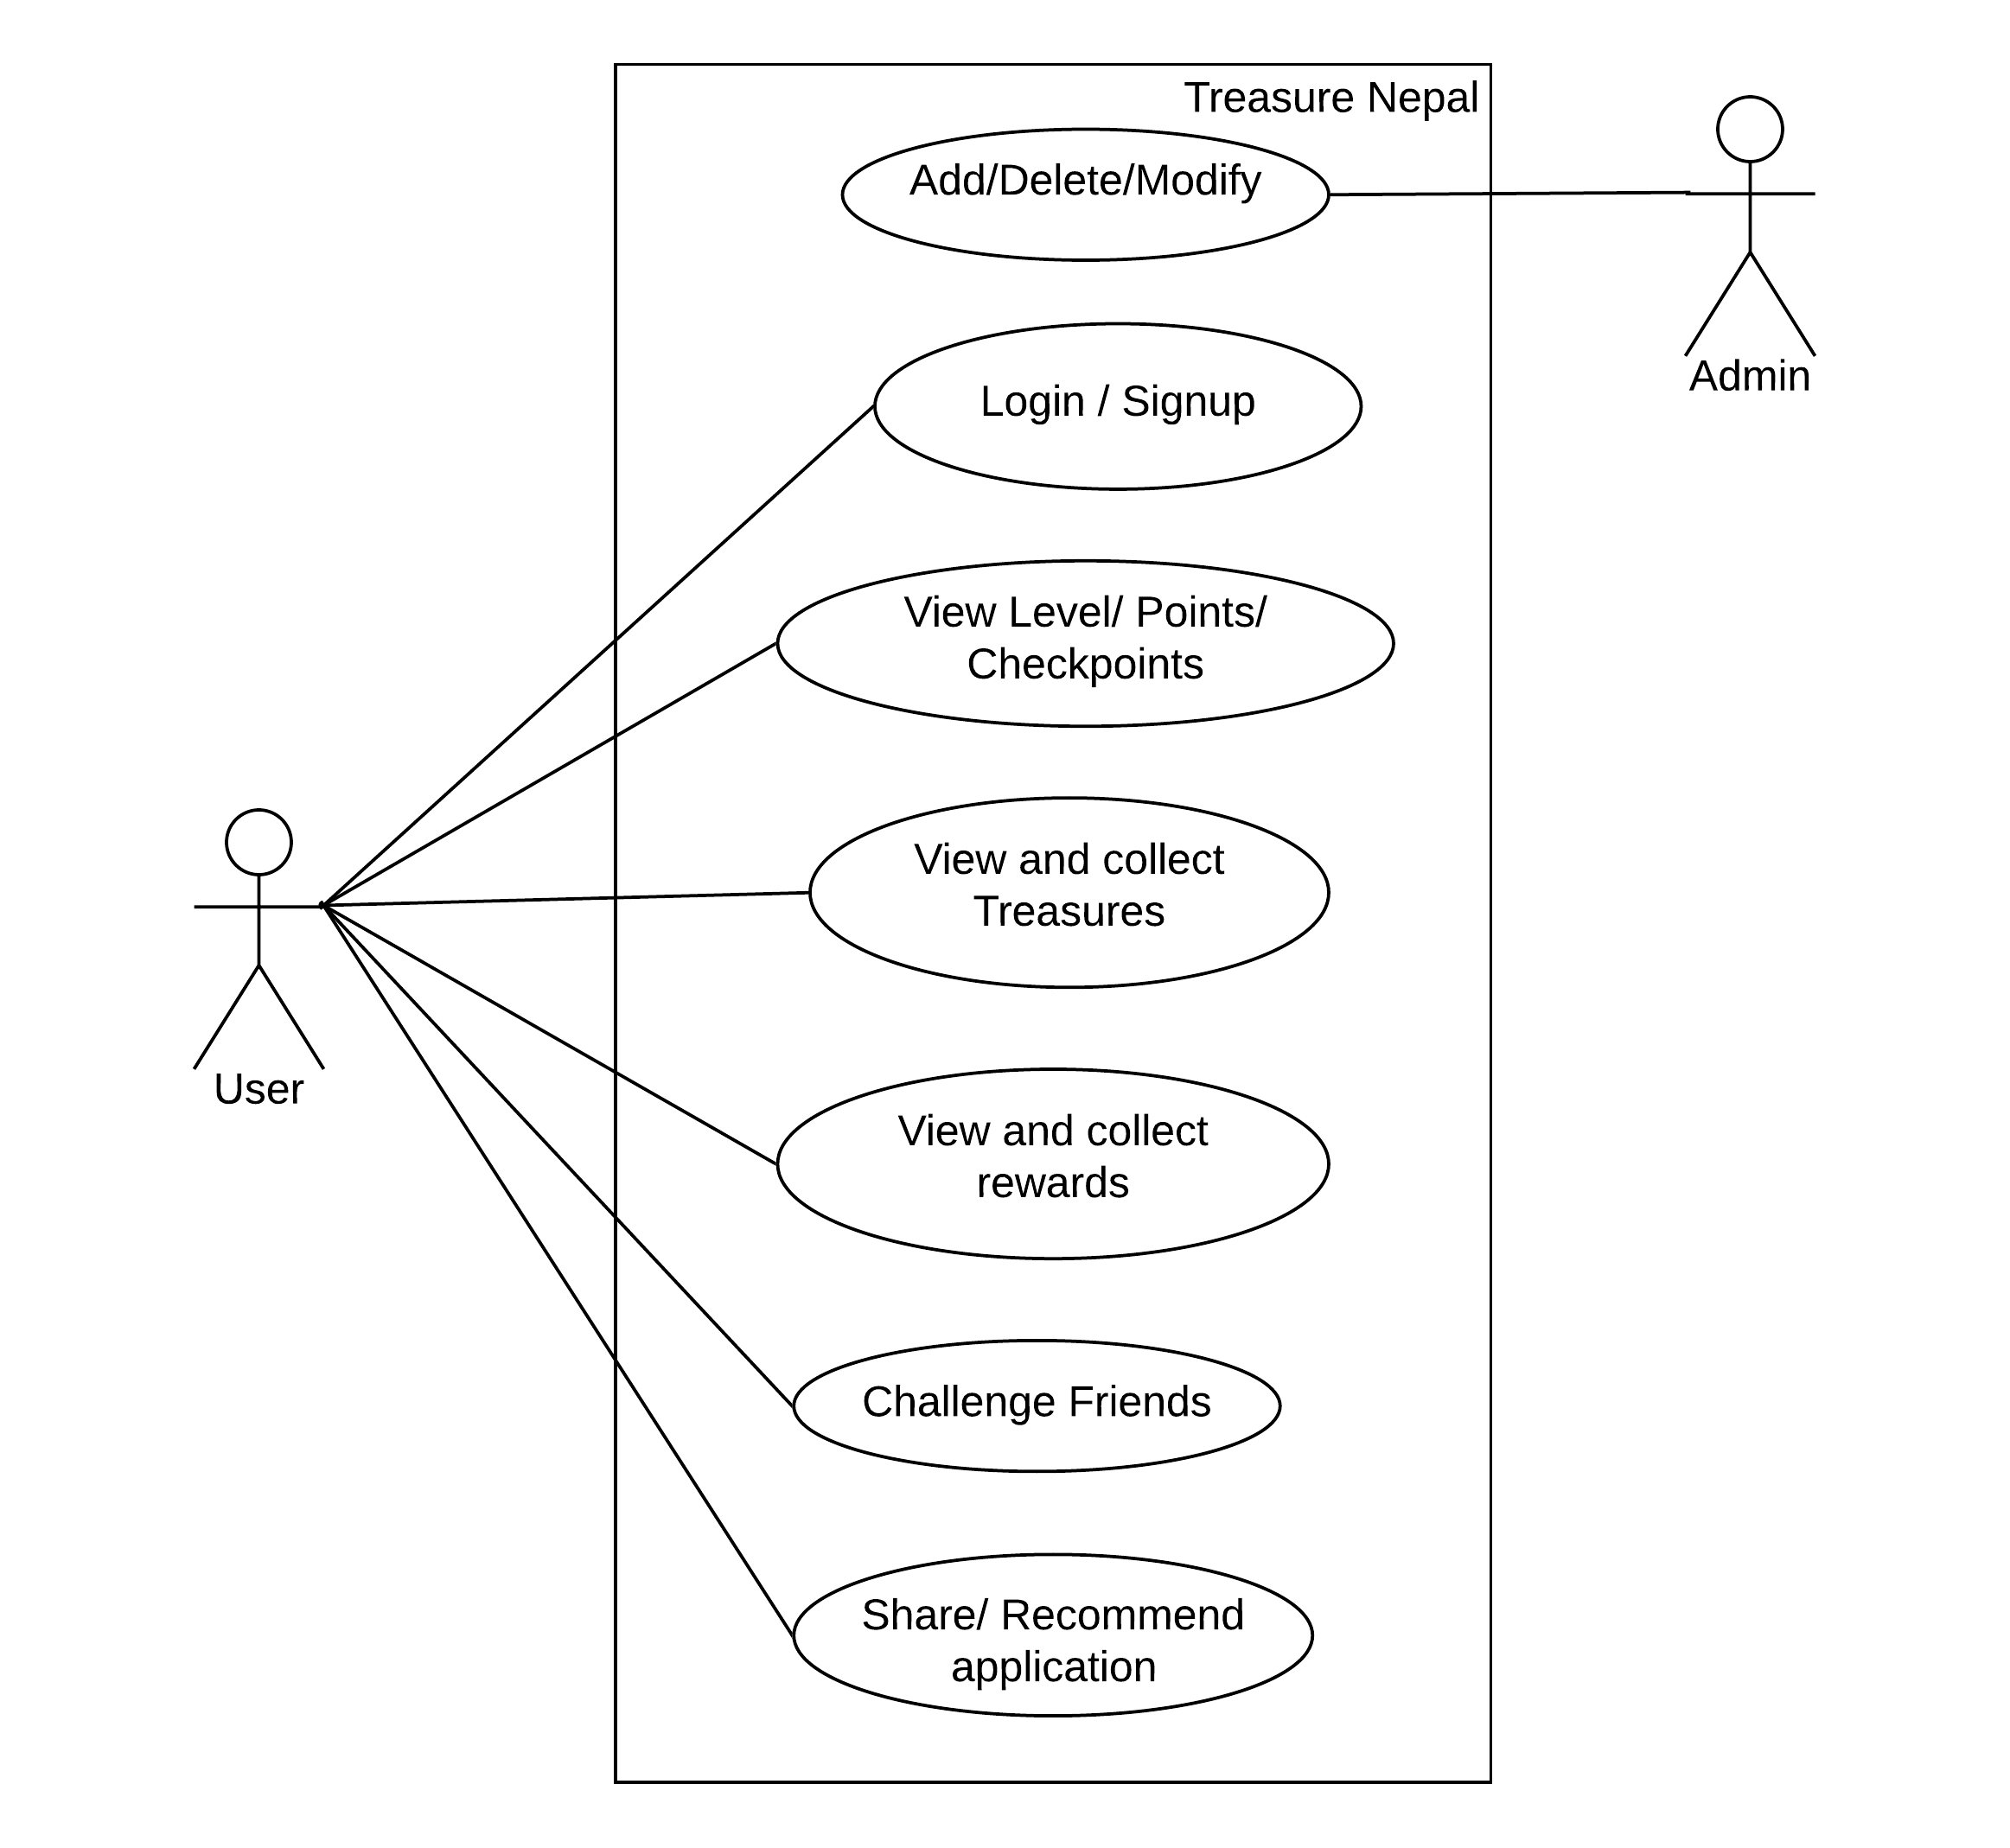
\includegraphics[width=\linewidth]{use-case-diagrams/all.png}
\centering
\caption{Use case diagram for overall application}
\label{fig:use-case-all}
\end{figure}

\vspace{200px}
This use case is prepared at the highest level of abstraction -- that is when the user uses the application as a whole. After a series of in depth analysis, we figured out that the two major parts in our application are the collection of treasures and rewards. So, we prepared use cases each for how a user would collect them.

\begin{table}[h!]
\centering
\begin{tabularx}{\linewidth}{|X|} 
\hline
\textbf{Use Case:  Treasure Collection}\\ 
\hline
After being logged in, the user can view all nearby treasure locations in a map. The user can also search treasures using name and location.  The user can also view information about the place she will be visiting in advance, and about the treasure available at that location. All the data related to the treasure are added and updated by an admin who has access to the database. When the user physically reaches the location where the treasure is installed, she uses the application to check in at that place. Based on the location of the place, the validity of collection is determined and the scores are attributed to the user. The user can write reviews about a particular treasure location and share it. She can also recommend to add some new places to the treasure database, which will be reviewed by the admin team.\\
\hline
\end{tabularx}
\end{table}

\begin{figure}[H]
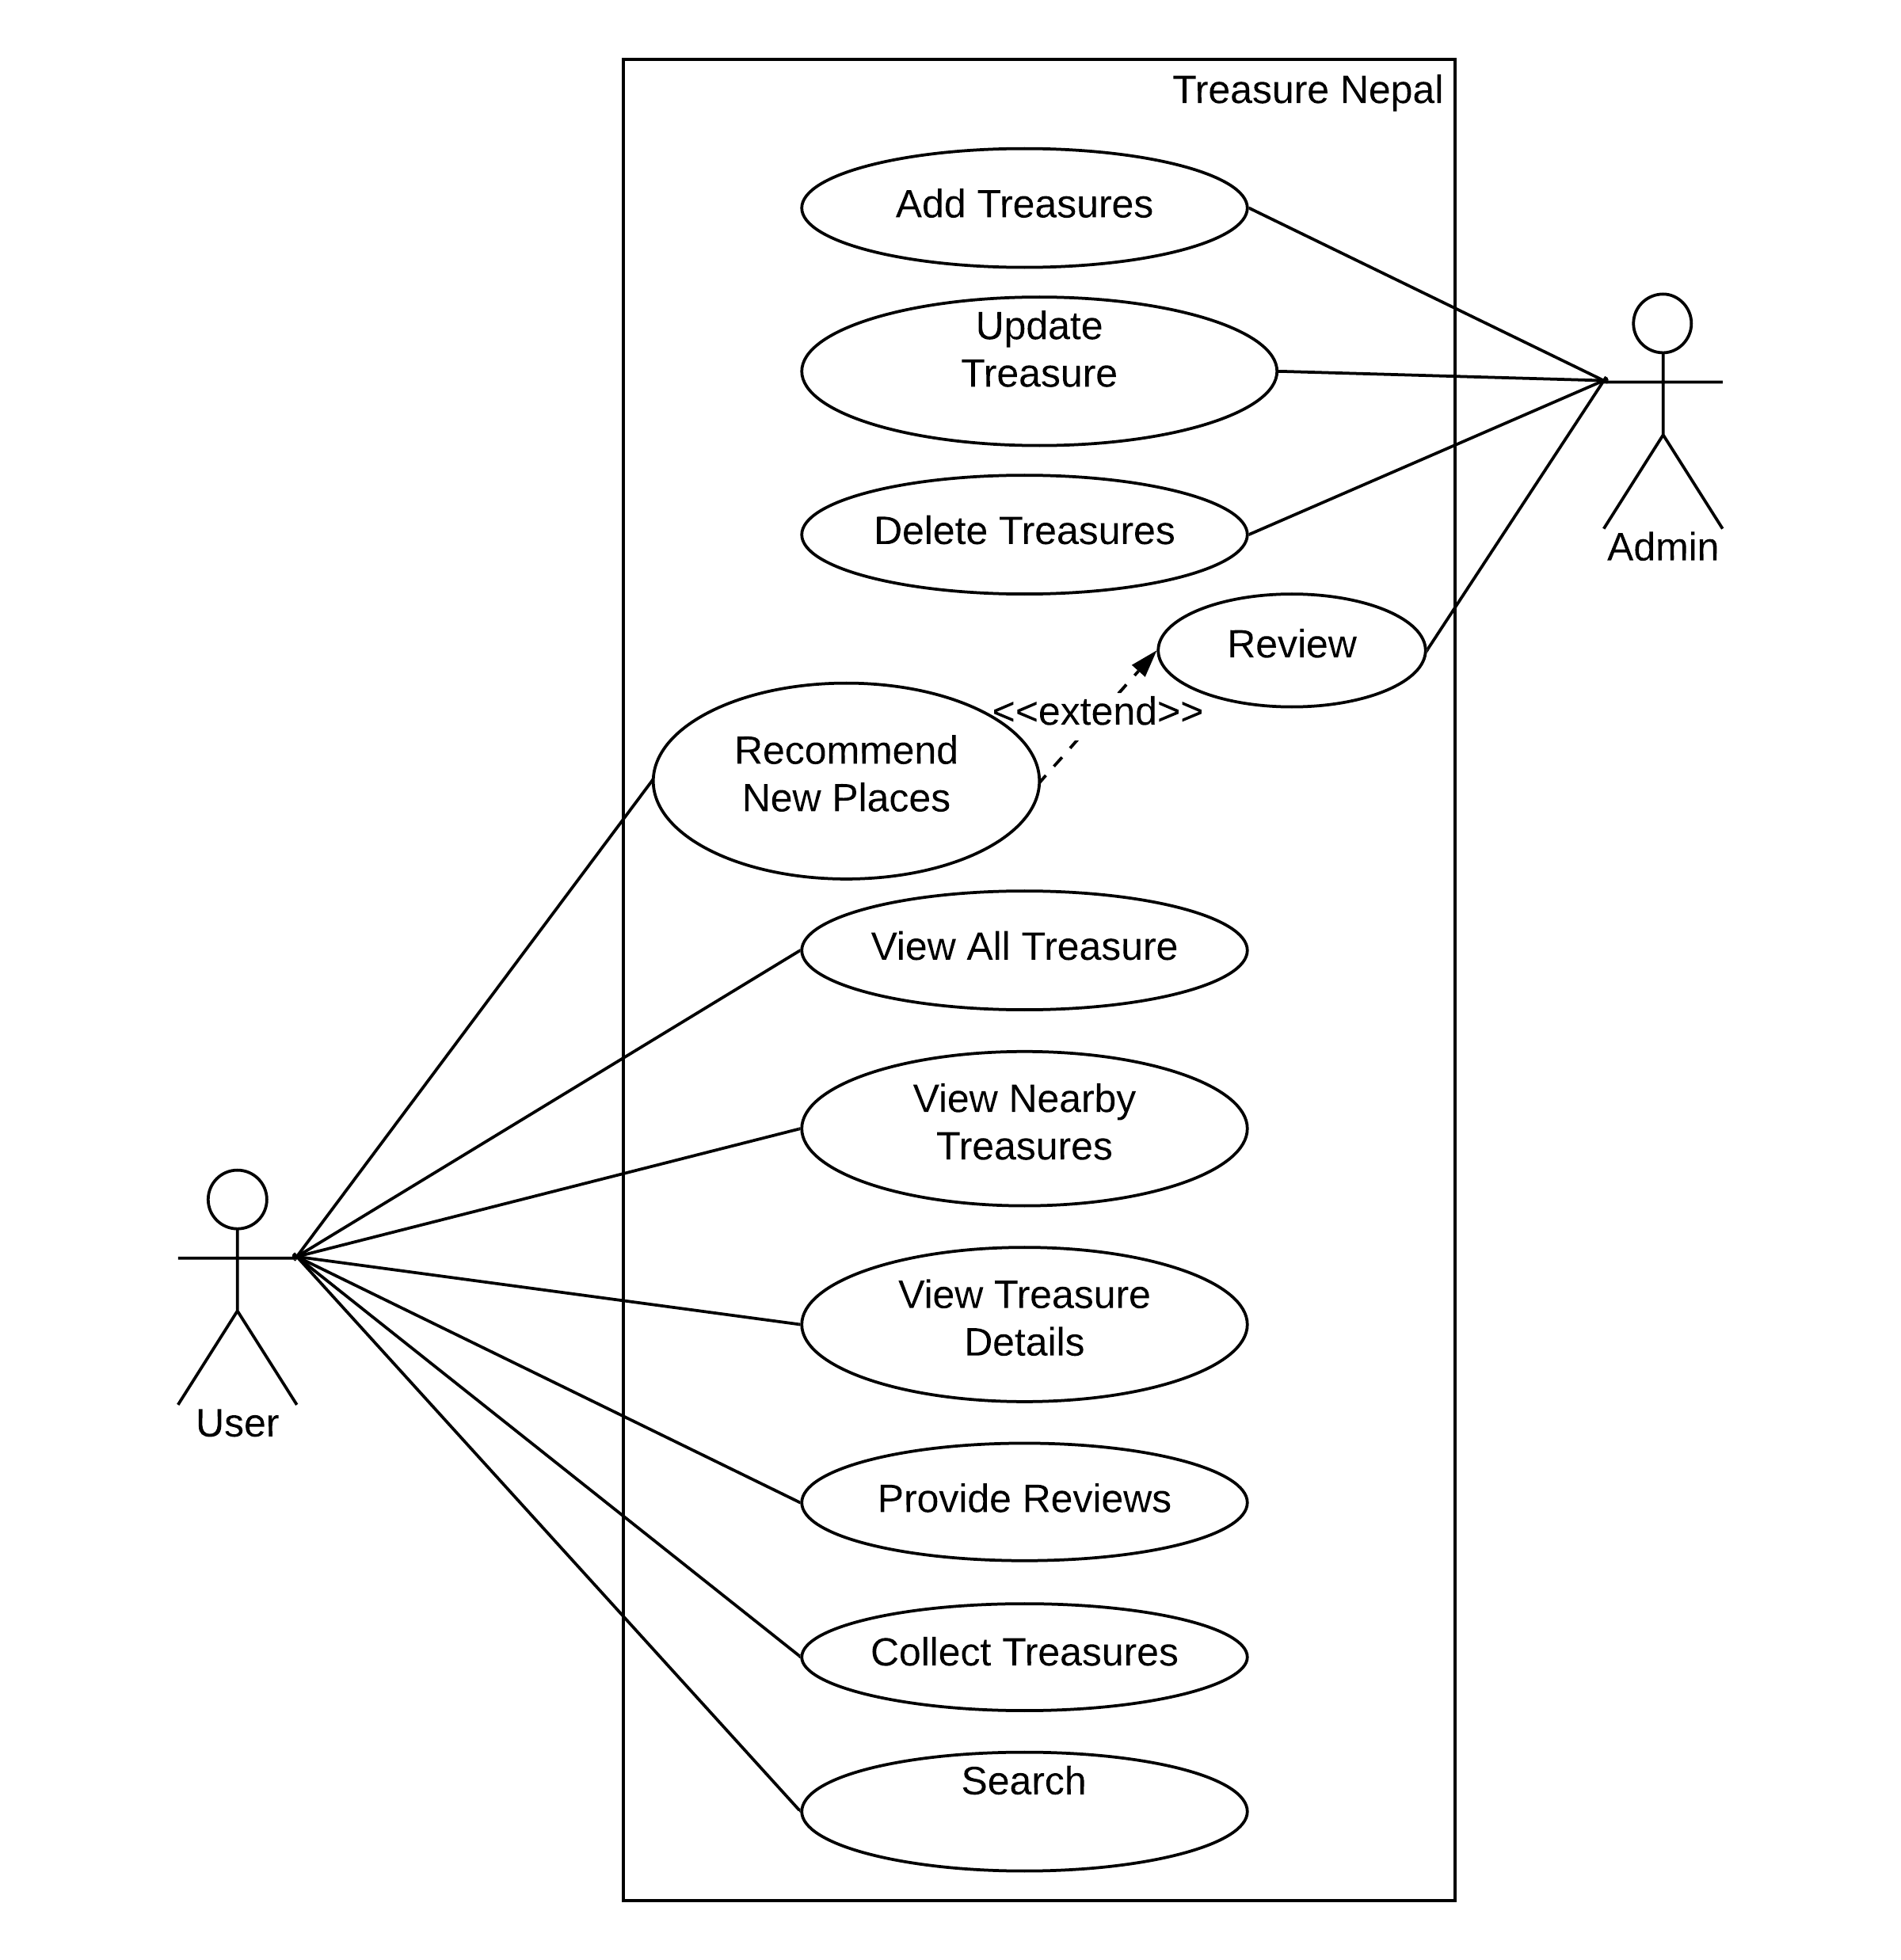
\includegraphics[width=\linewidth]{use-case-diagrams/treasure.png}
\centering
\caption{Use case diagram for treasure collection}
\label{fig:use-case-treasure}
\end{figure}

\vspace{200px}

\begin{table}[H]
\centering
\begin{tabularx}{\linewidth}{|X|} 
\hline
\textbf{Use Case:  Reward Collection}\\ 
\hline
The application will have a number of rewards and offers from different business partners like hotels, resorts, restaurants, etc. The eligibility of a user to claim these rewards will be based on their points. After the points cross a certain level, several of the rewards will be unlocked. To redeem those awards, the user have to visit the reward location, and scan QR code at that location. An admin will be responsible for adding and updating the rewards and offers in the central database. She will also be able to provide reviews and ratings to the rewards she collects.\\
\hline
\end{tabularx}
\end{table}

\begin{figure}[H]
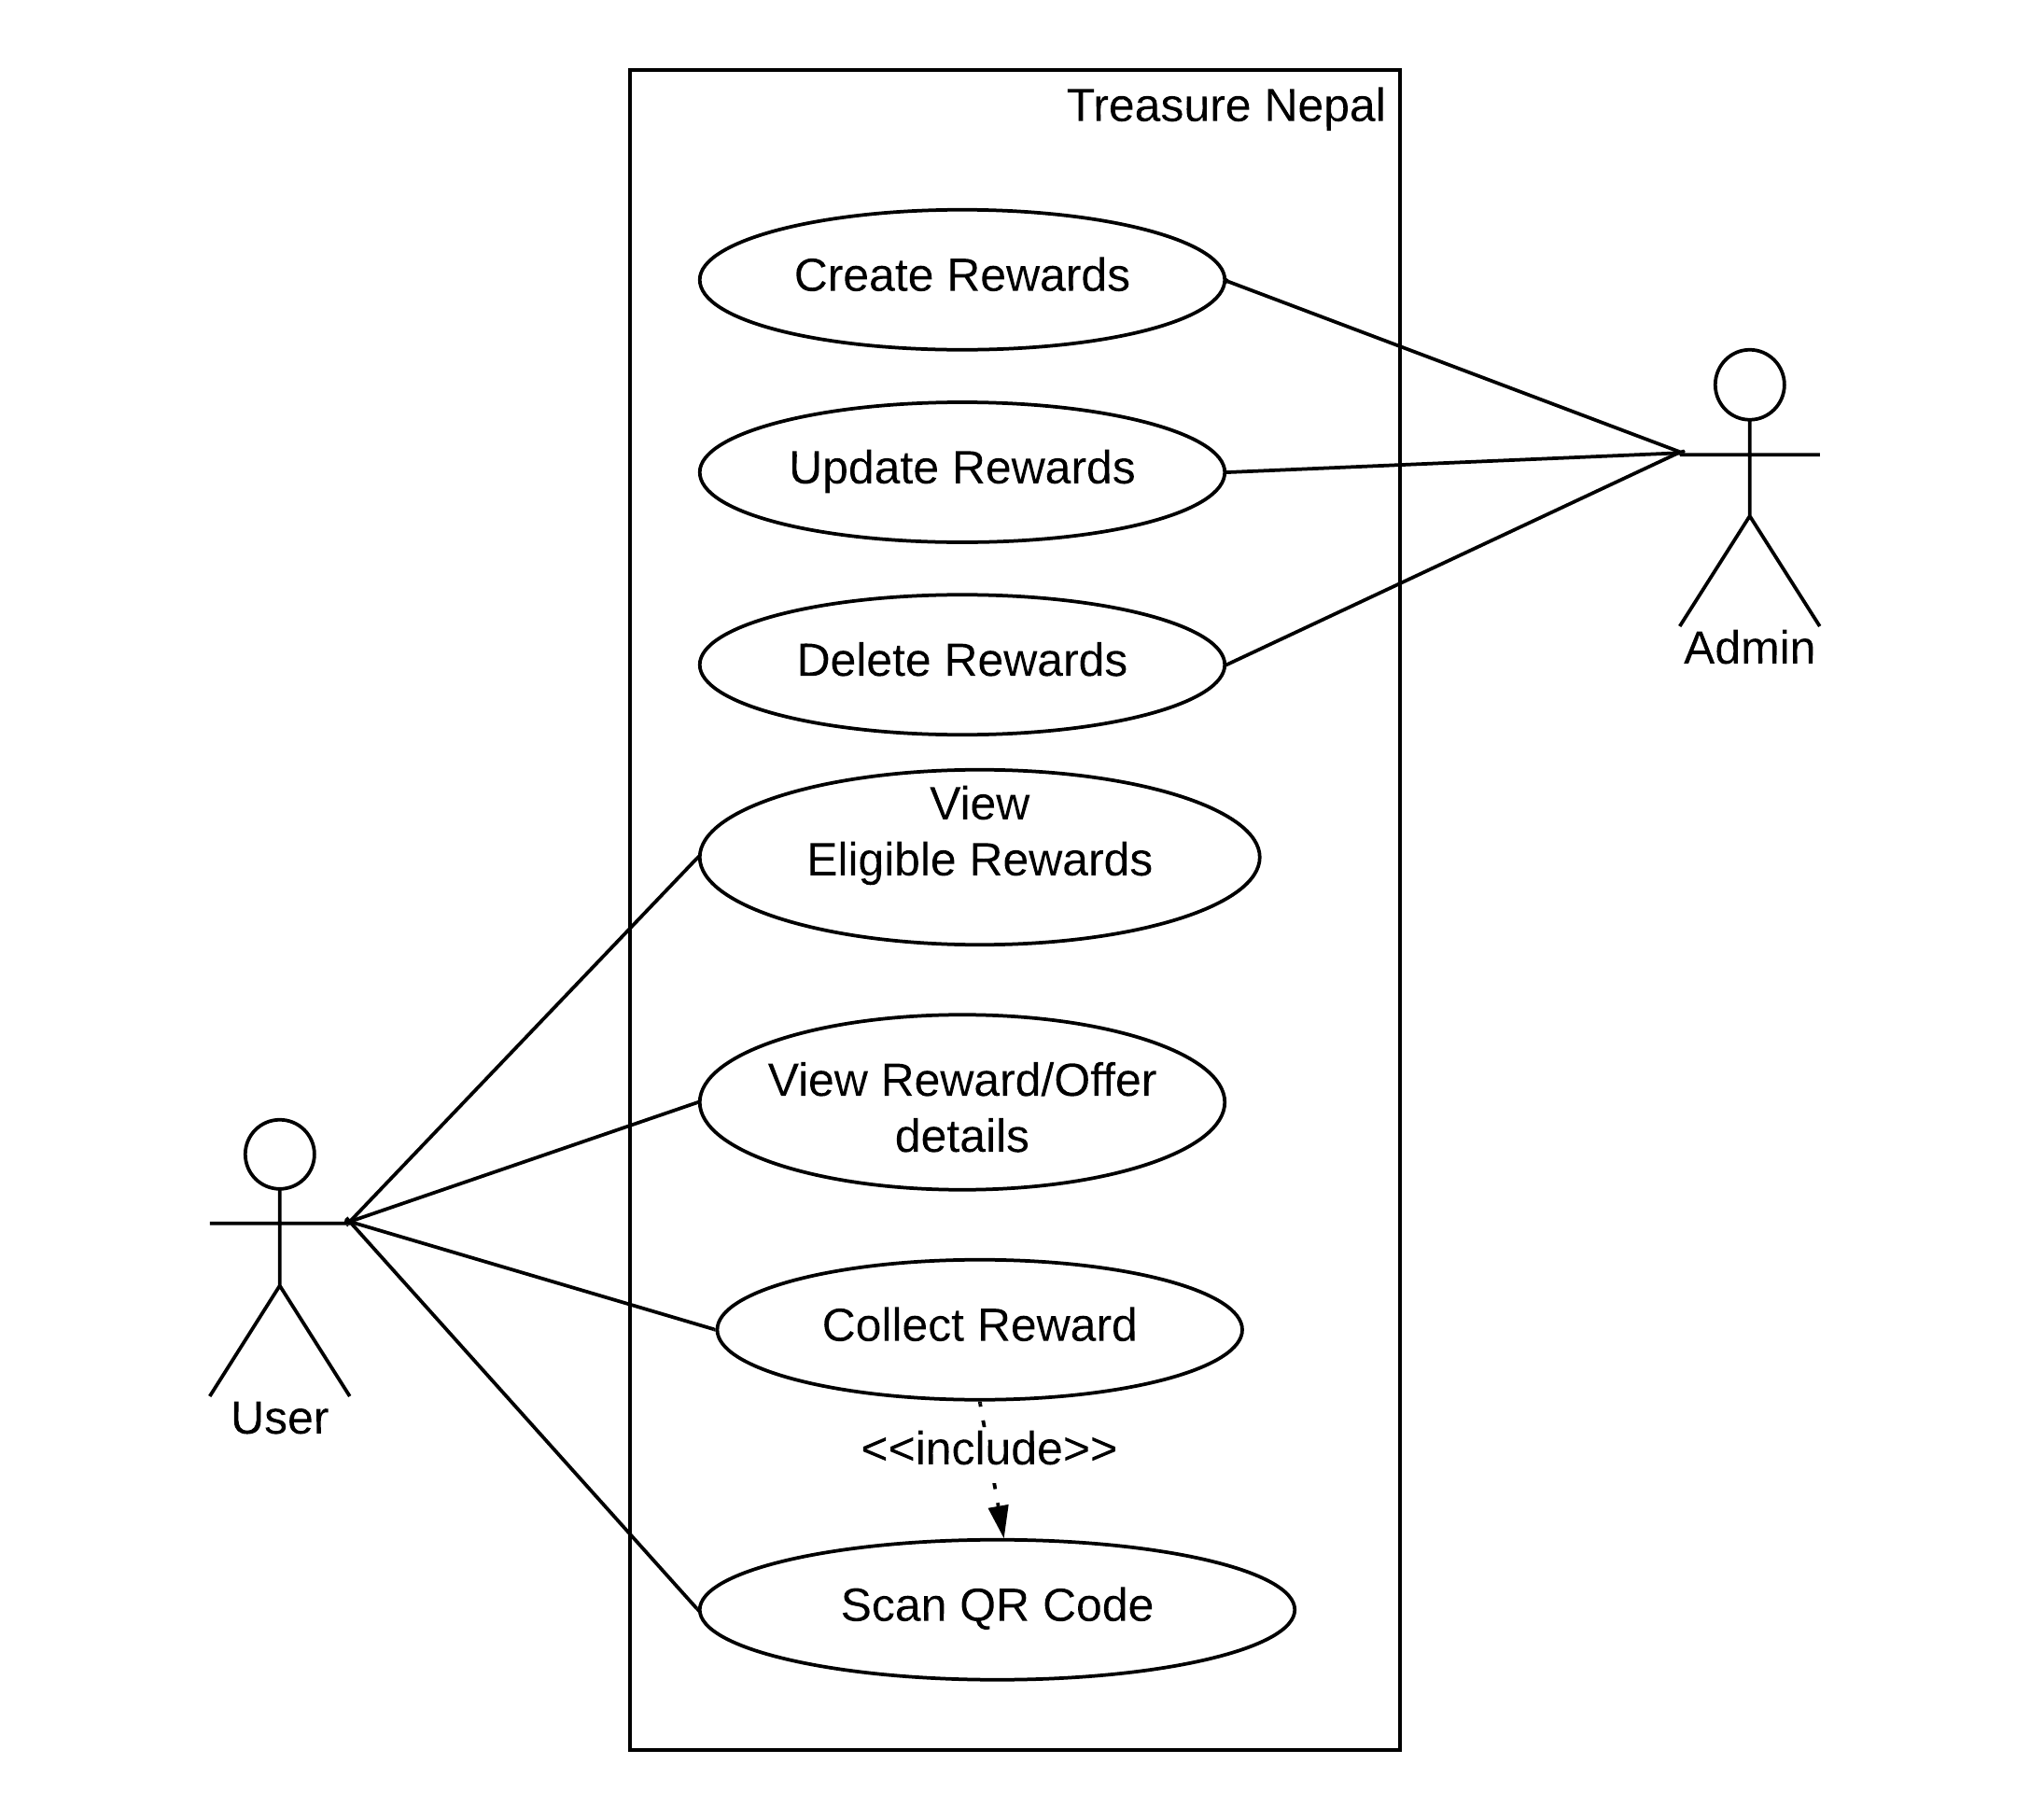
\includegraphics[width=\linewidth]{use-case-diagrams/reward.png}
\centering
\caption{Use case diagram for reward collection}
\label{fig:use-case-reward}
\end{figure}

\subsection{Database Design}
The following class diagram illustrates the database schema used for the application. 

\begin{figure}[H]
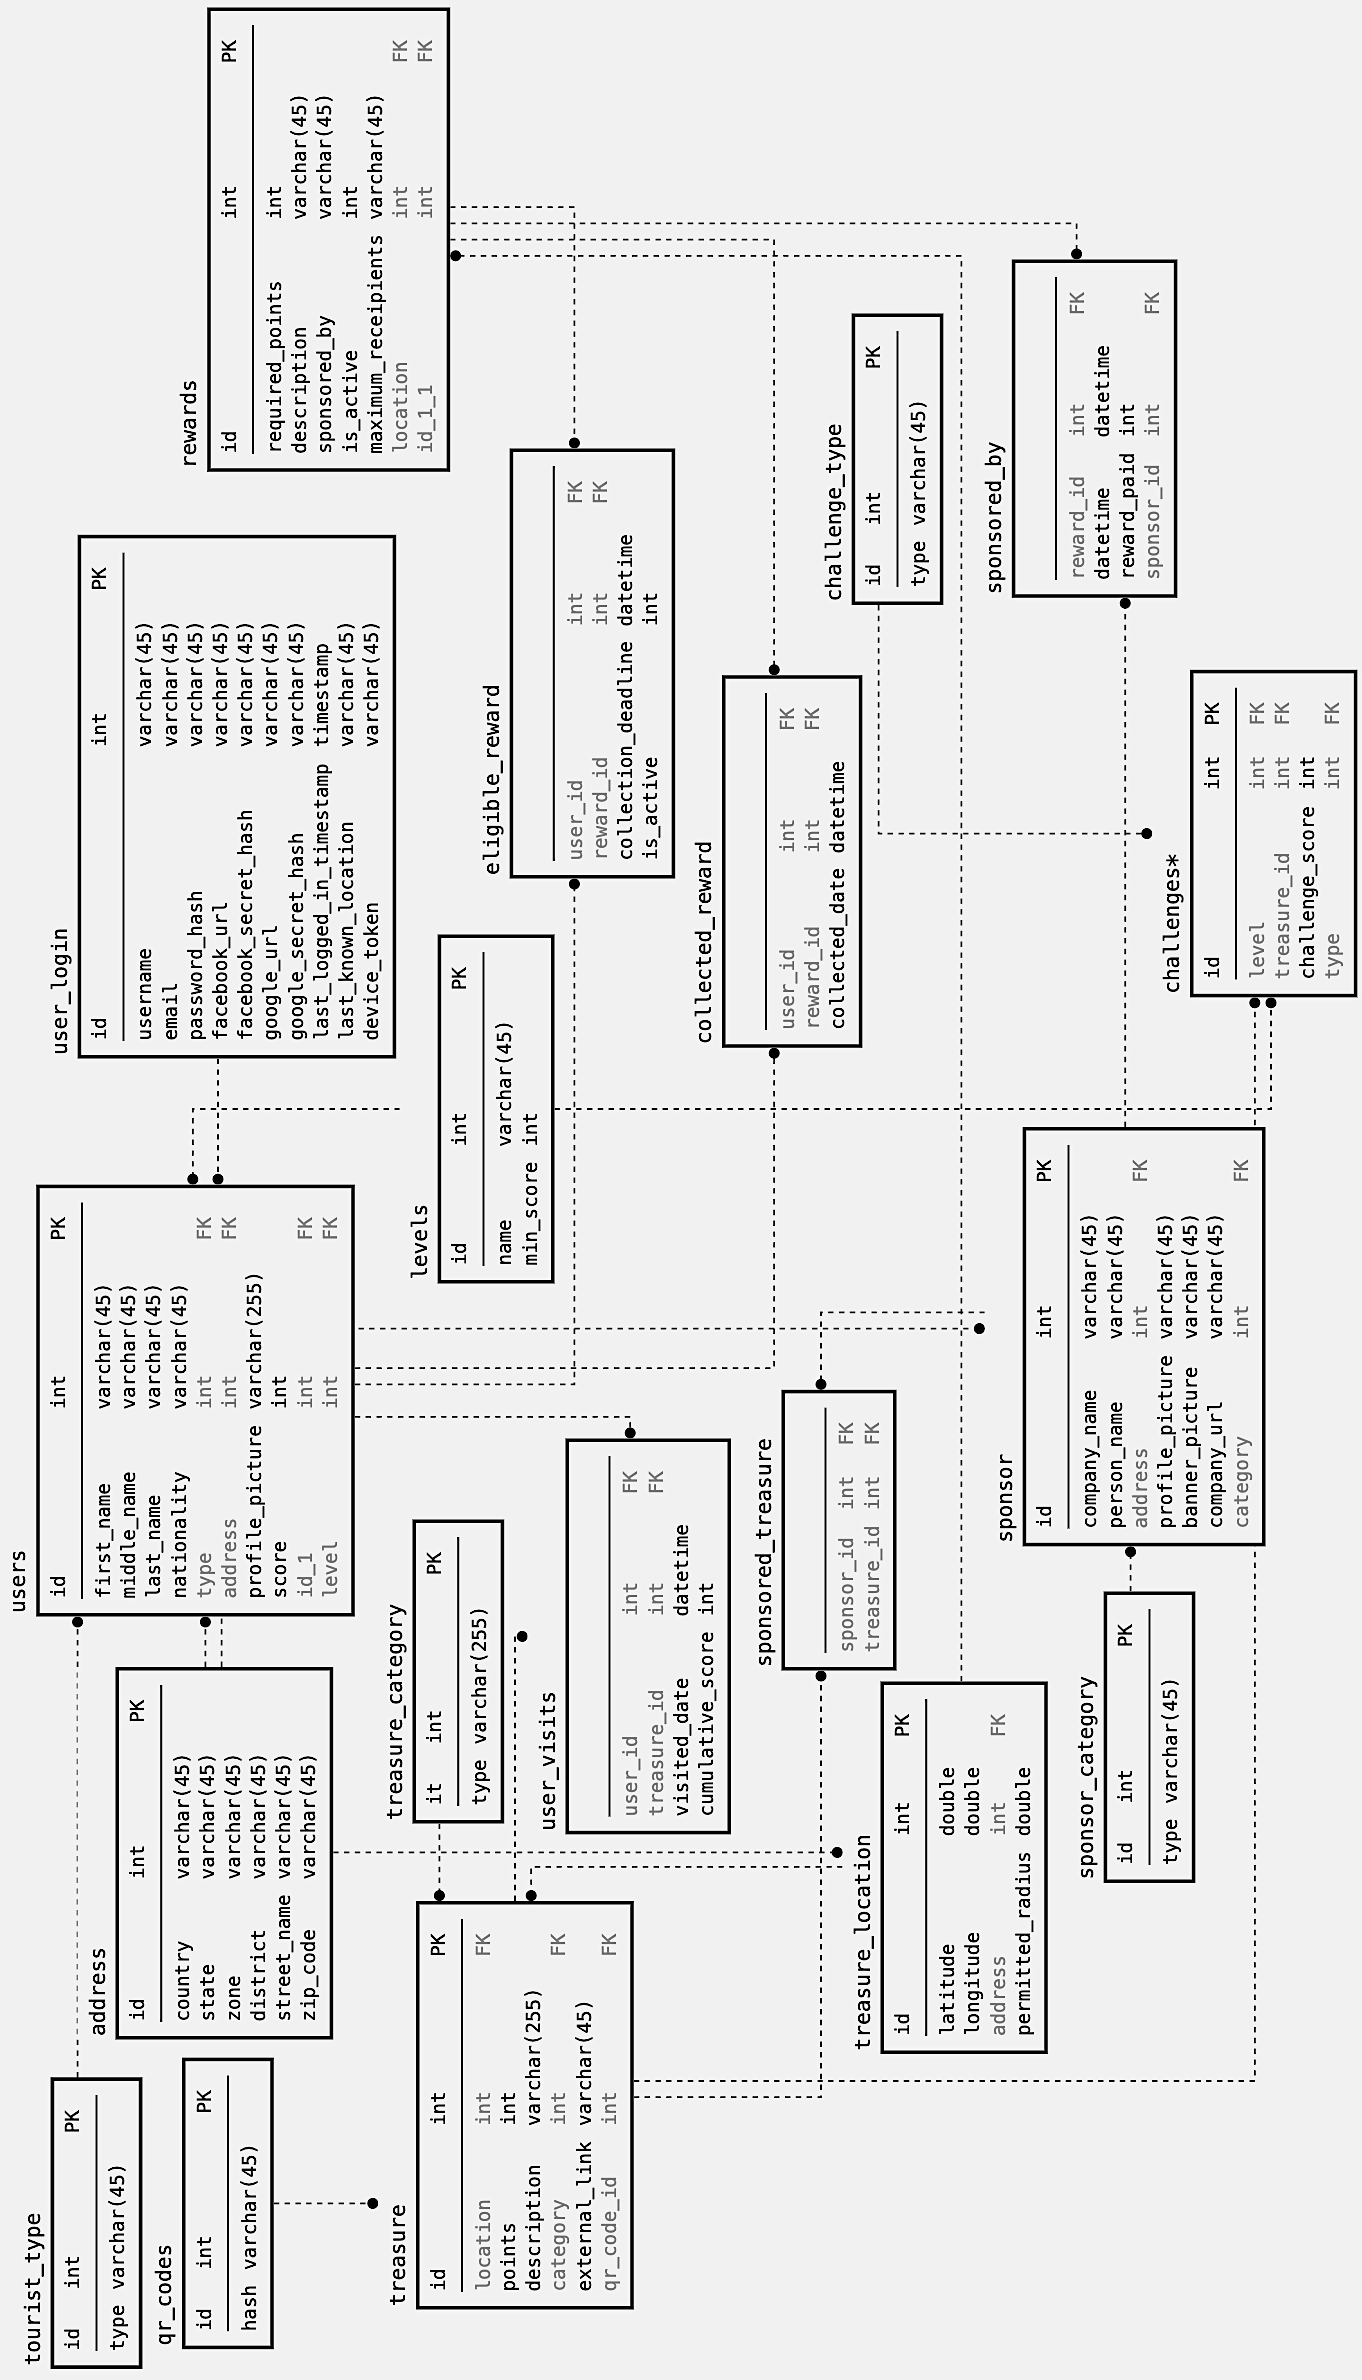
\includegraphics[height=0.8\paperheight, keepaspectratio]{db/schema.png}
\centering
\caption{Schema used in backend database}
\label{fig:db-schema}
\end{figure}

The database used for the API backend in the project is MySQL. Since the mobile applications do not access the data directly from the database, the API server is responsible for fetching the data in accordance to the API query and send it to the mobile device. 

\subsection{Data Collection}
Our team has collected data about the various tourist destinations and places (the data include the location, the photos, latitude, longitude, how to get to that place, entry fee, etc.) so that we can add treasures to those places and add them to our database.

The following figure shows a sample of data collected by our team.


\begin{figure}[H]
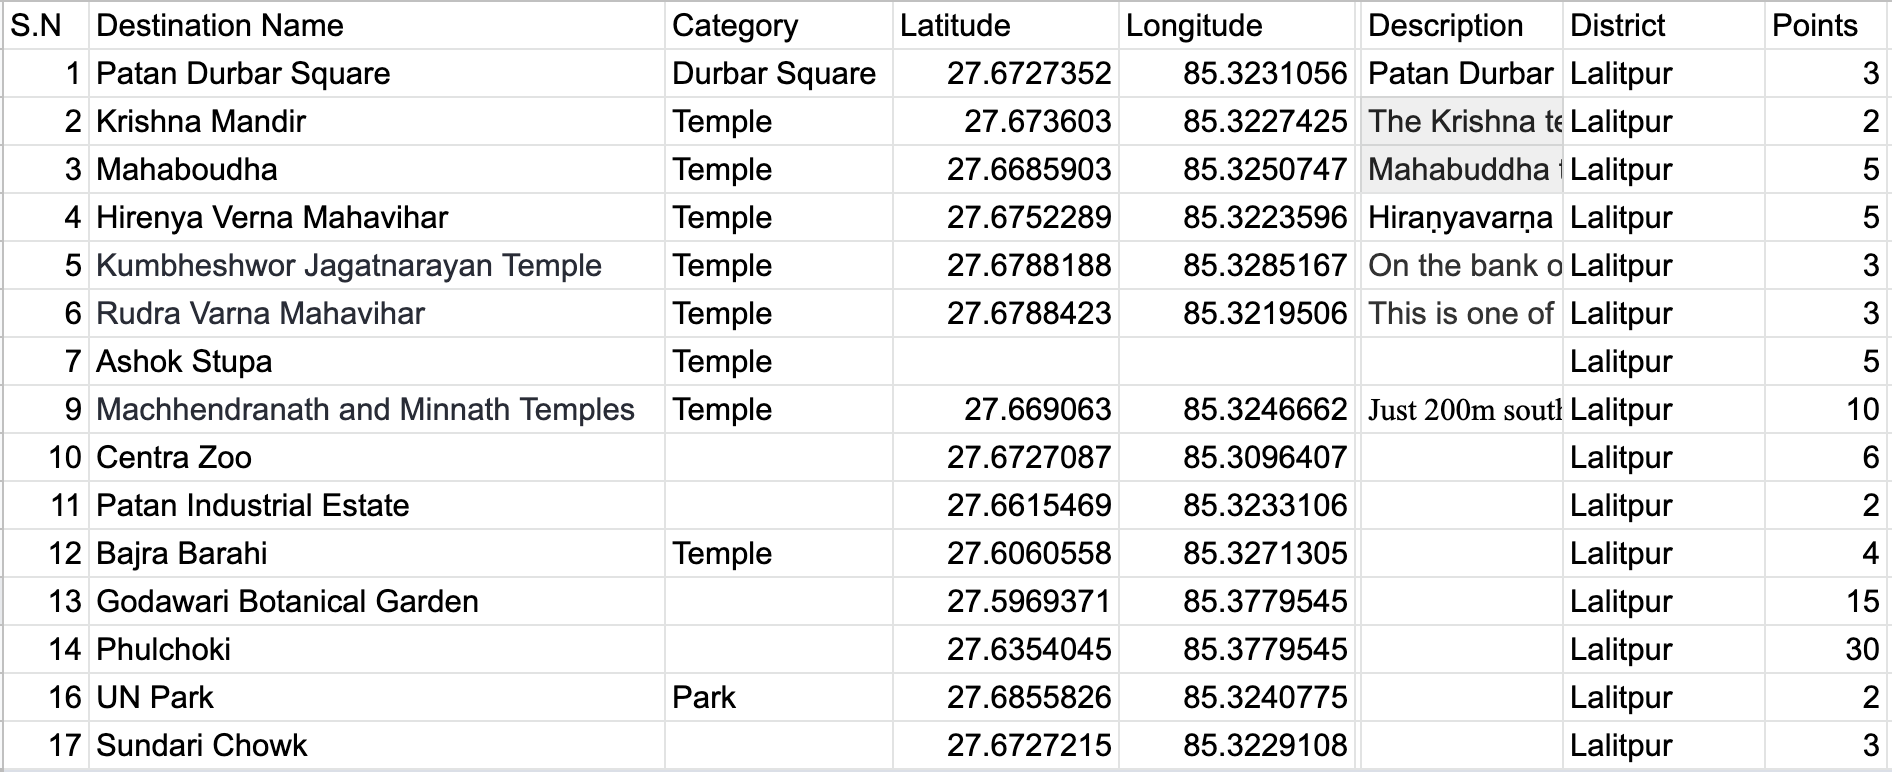
\includegraphics[width=\linewidth, keepaspectratio]{screenshots/data-collection.png}
\centering
\caption{Model of data collection}
\label{fig:data-model}
\end{figure}


\subsection{Backend API}
The API endpoints for creating, updating, reading and deleting the data from all of the tables shown in Figure \ref{fig:db-schema} have already been created. The following table shows the syntax of different endpoints of the API.


\begin{table}[H]
\begin{tabularx}{\linewidth}{|c|c|c|X|}
\hline
\rowcolor[HTML]{C0C0C0} 
\textbf{Endpoint}                & \textbf{Method} & \textbf{Body}        & \textbf{Response}                                               \\ \hline
/\{table\_name\}        & GET    & -           & List of all data entries in the table                  \\ \hline
/\{table\_name\}/\{id\} & GET    & -           & The entry in the table corresponding to provided ID    \\ \hline
/\{table\_name\}/       & POST   & data object & Entry for data object created in the database          \\ \hline
/\{table\_name\}/\{id\} & PUT    & data object & Update the entry with provided id with new data object \\ \hline
/\{table\_name\}/\{id\} & DELETE & -           & Delete the entry corresponding to the provided id      \\ \hline
\end{tabularx}
\end{table}

The following figure shows an instance of API request and response.

\begin{figure}[H]
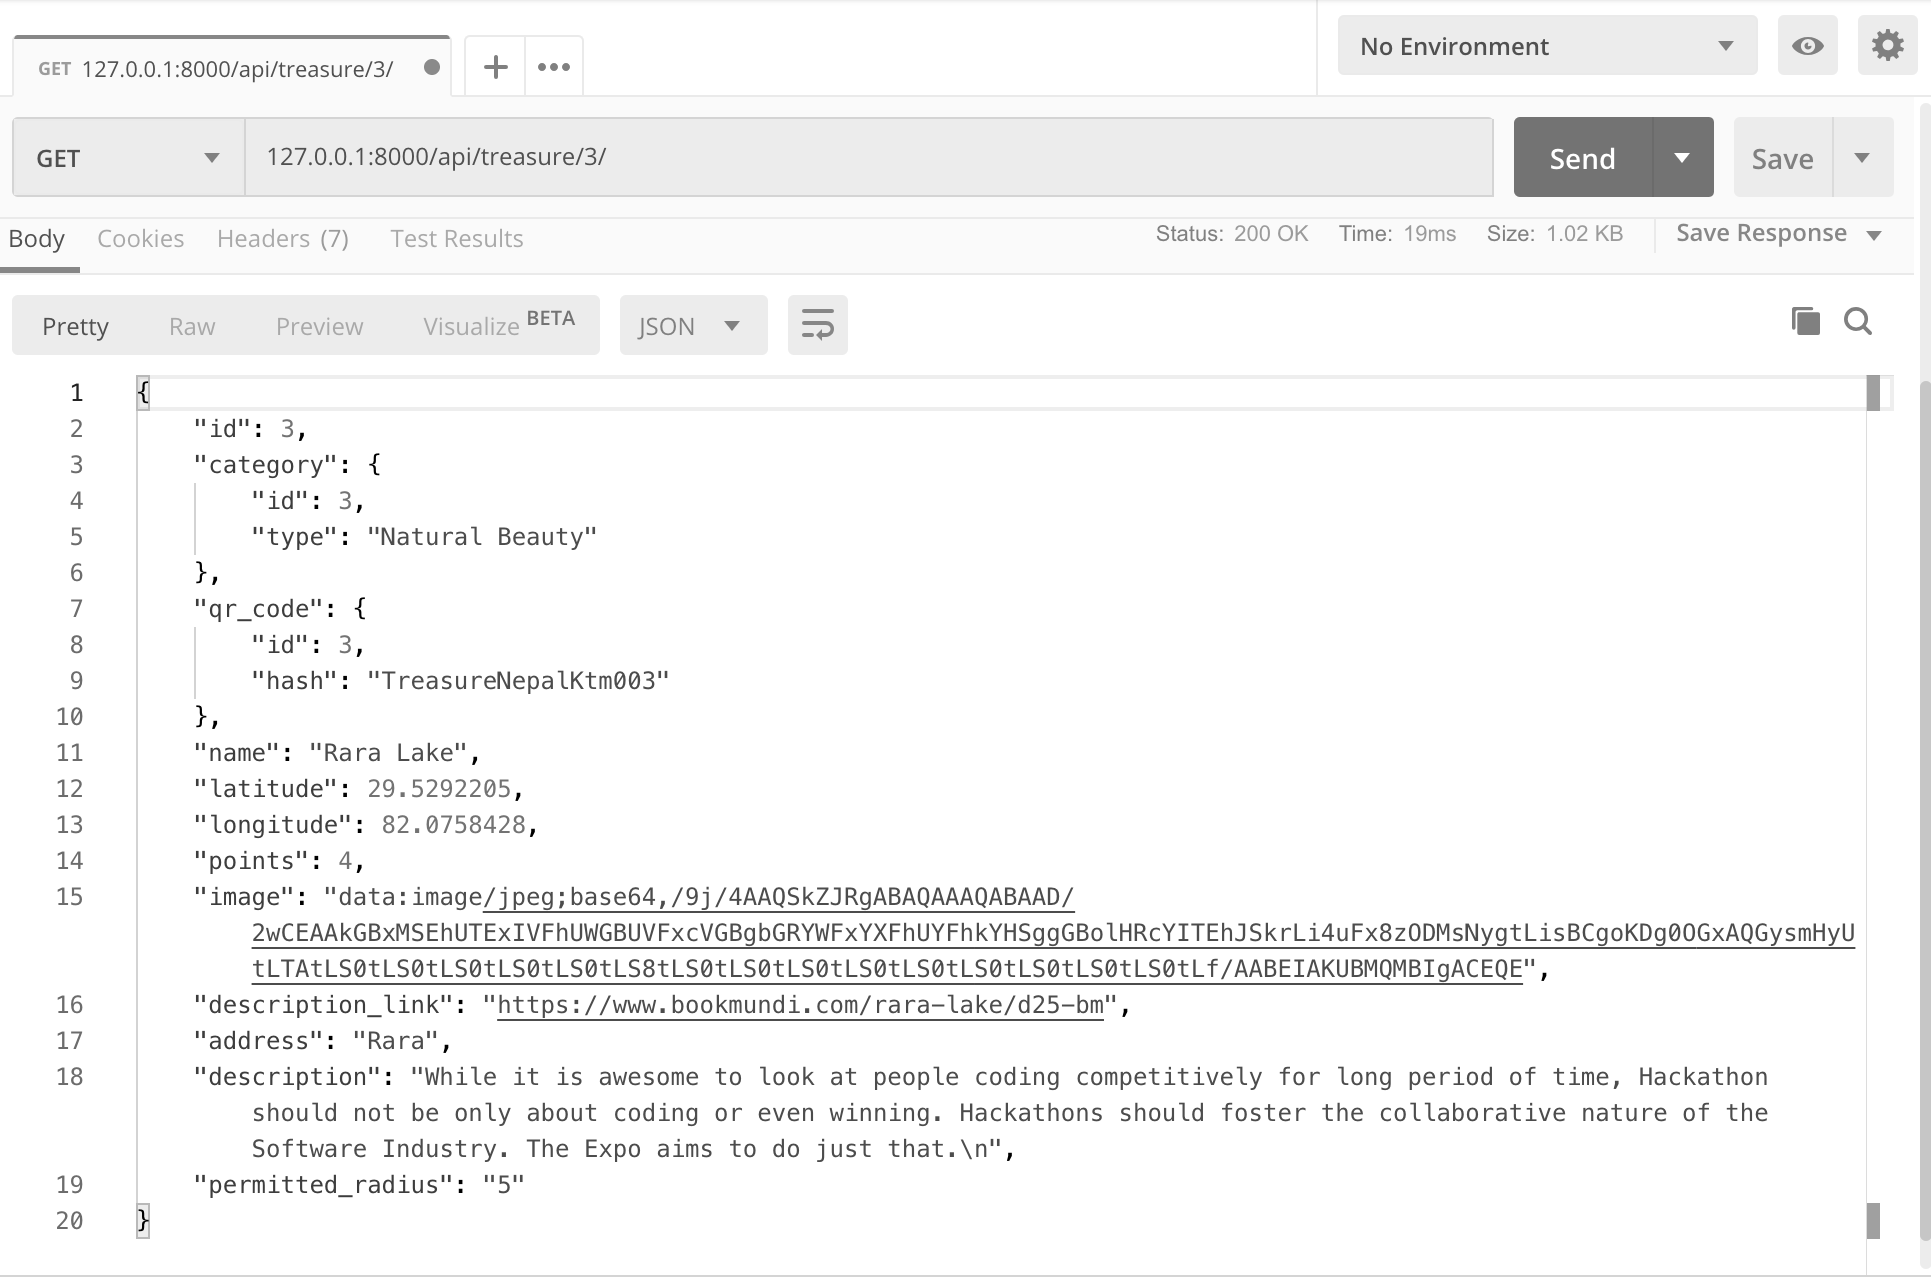
\includegraphics[width=\linewidth, keepaspectratio]{screenshots/api.png}
\centering
\caption{Screenshot of API request and response using Postman}
\label{fig:auth-sequence}
\end{figure}


\subsection{Authentication Module}
The user authentication module has been completed in the backend, using email, Facebook as well as Google. In the backend, we have use django-rest-auth module for authentication management. This gives the user a unique api key whenever she logs in to the application. The user should then include that key in every request she sends to the API server.

The following sequence diagram shows how a user authenticates with the application.

\begin{figure}[H]
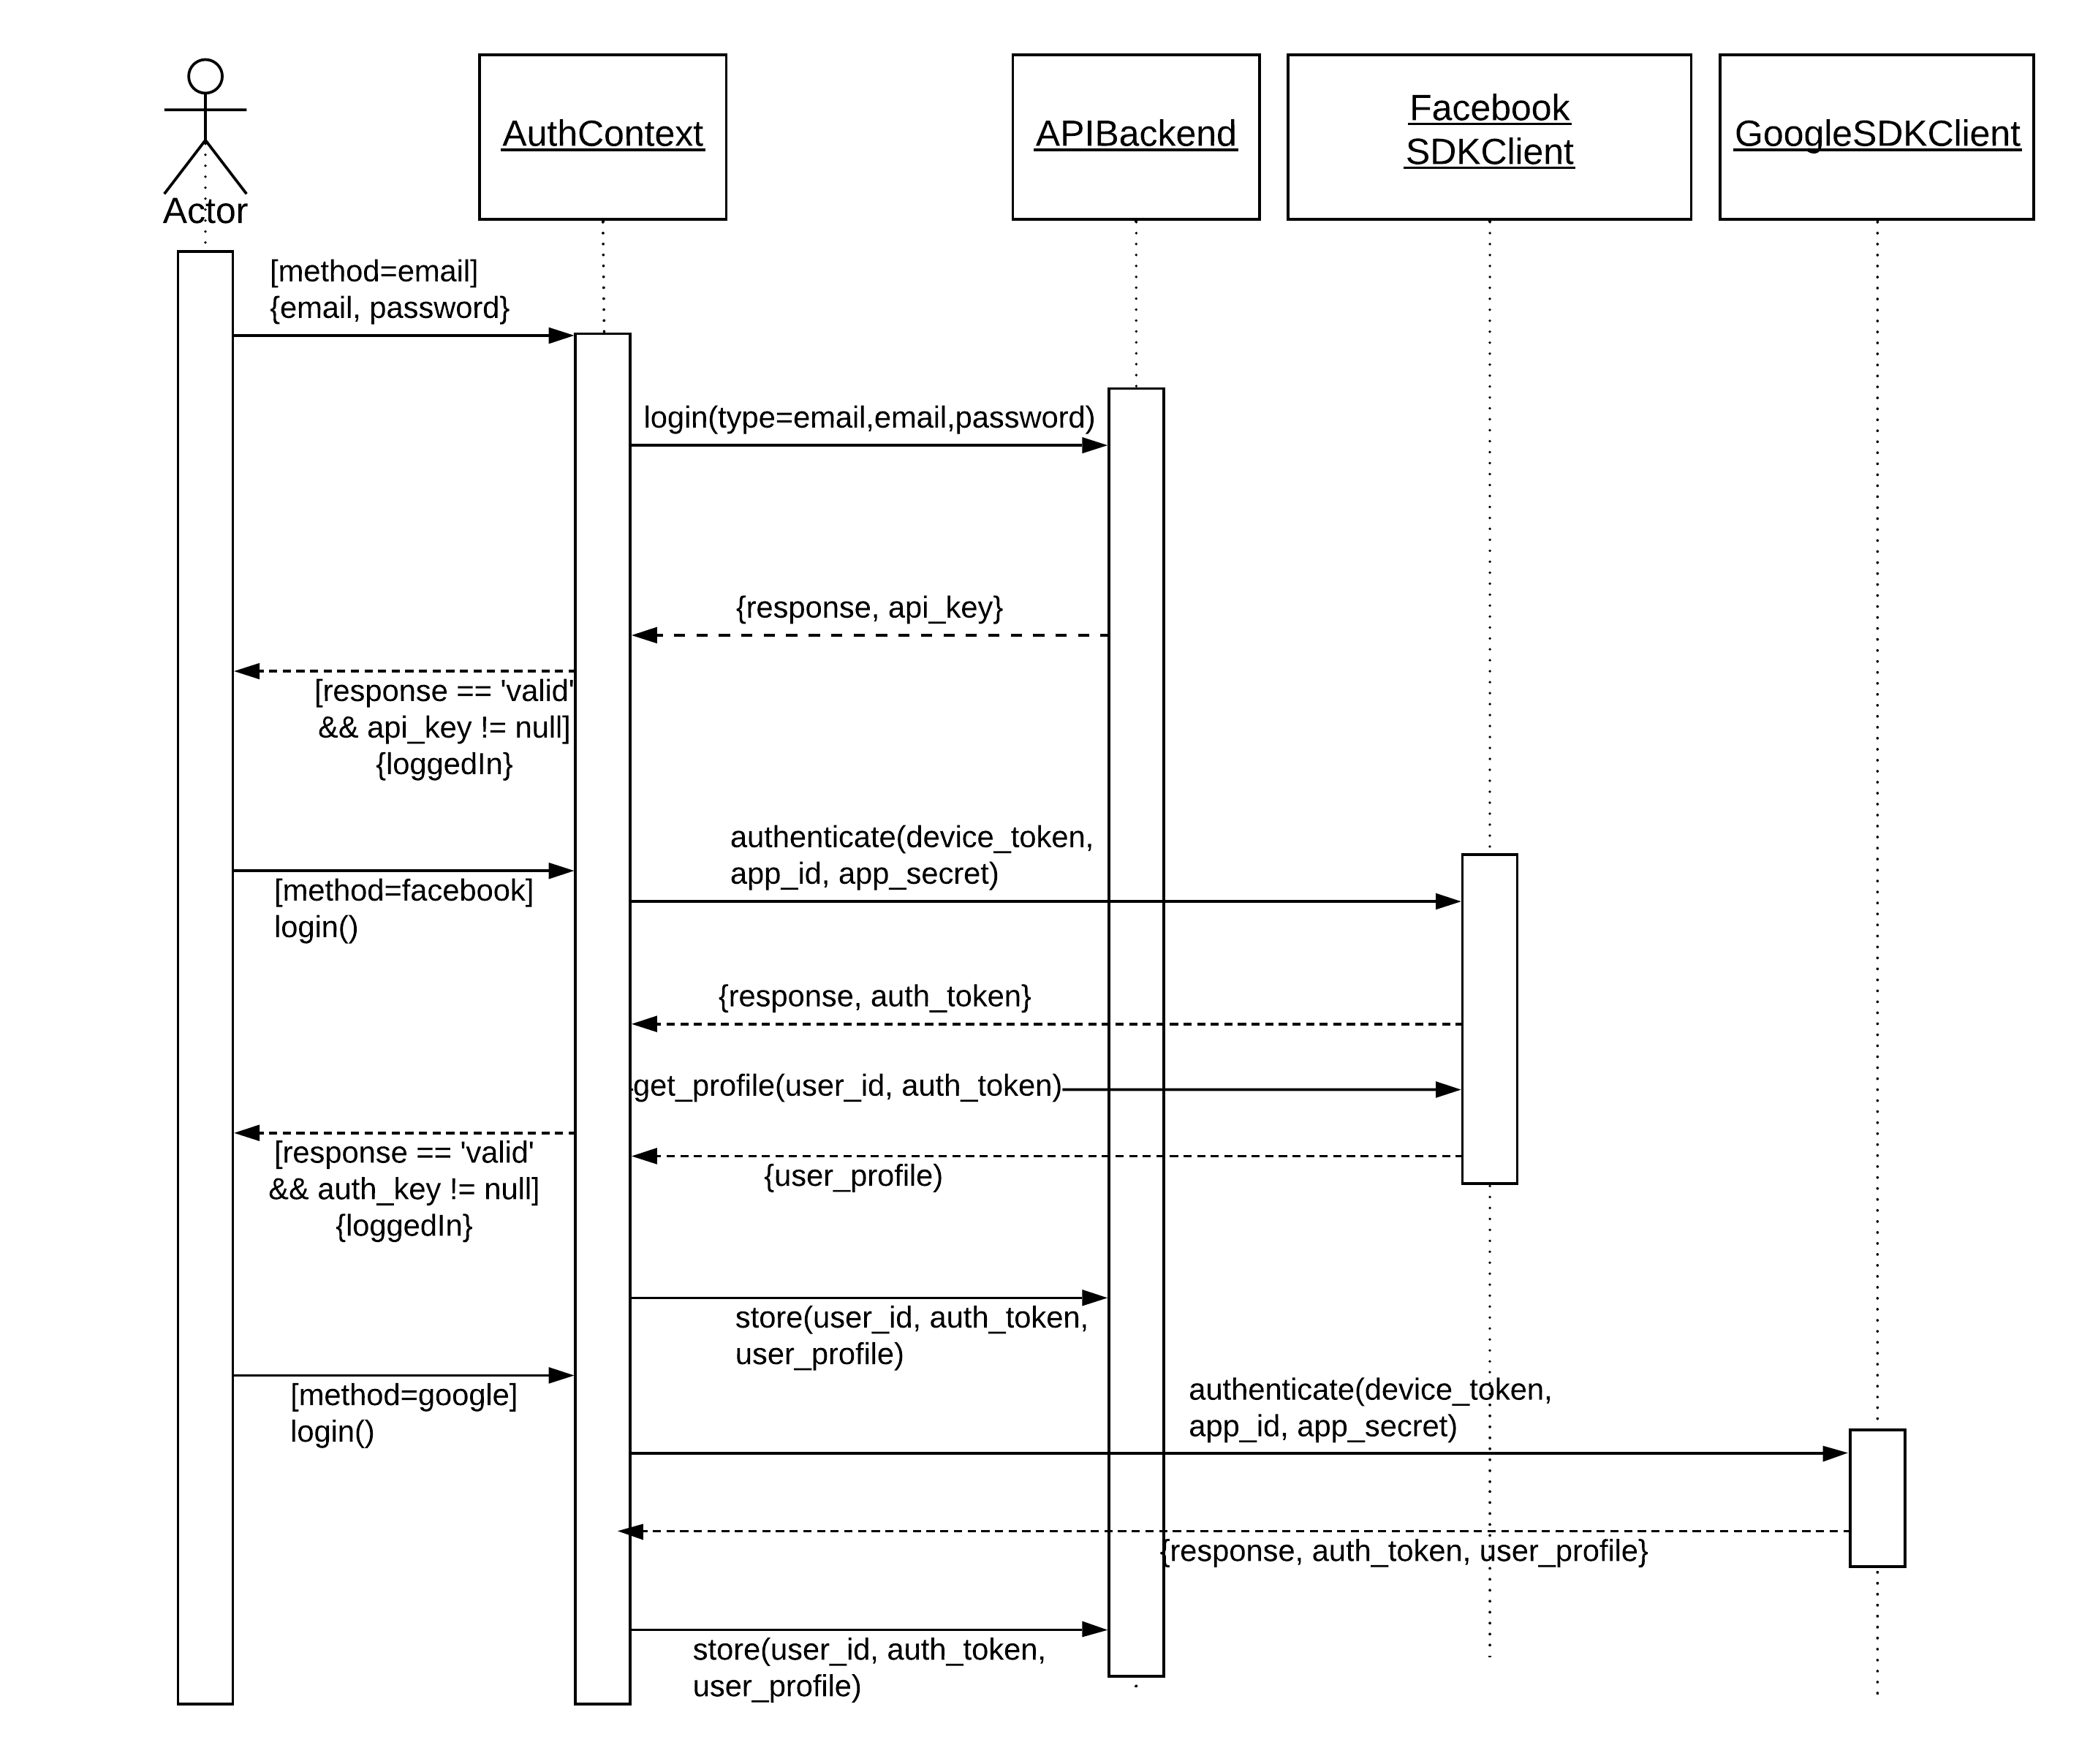
\includegraphics[width=\linewidth, keepaspectratio]{sequence-diagrams/auth.png}
\centering
\caption{Sequence diagram for user authentication}
\label{fig:auth-sequence}
\end{figure}

\subsection{Application Development}
The authentication has been integrated in the application development and as of now, it is fully working in both Android and iOS devices. The user can successfully login and out either using email, Facebook or Google sign in options.

The following figures show some screenshots of the application developed so far.

\begin{figure}[H]
\centering
	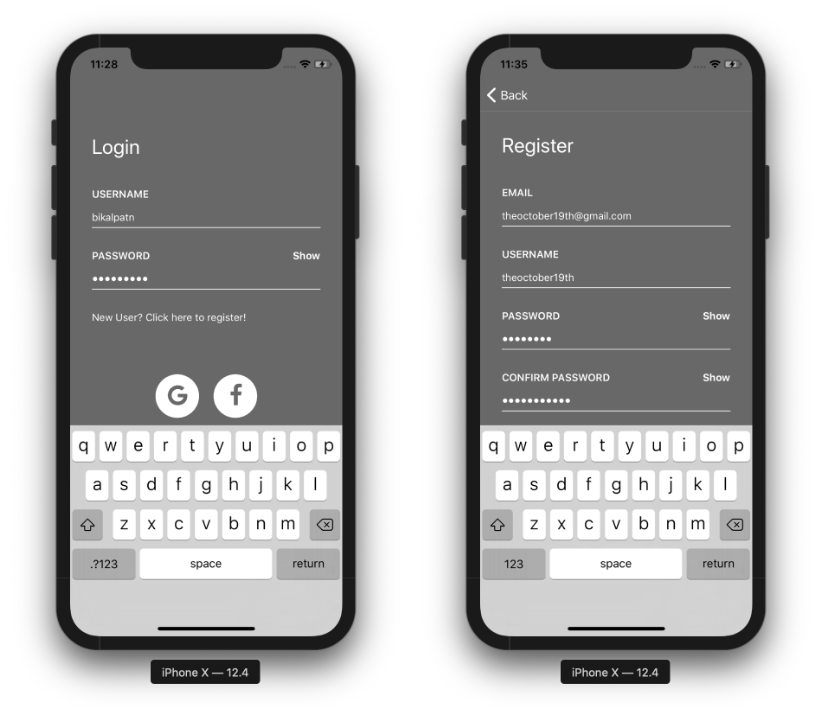
\includegraphics[width=\linewidth]{screenshots/1.png}	
	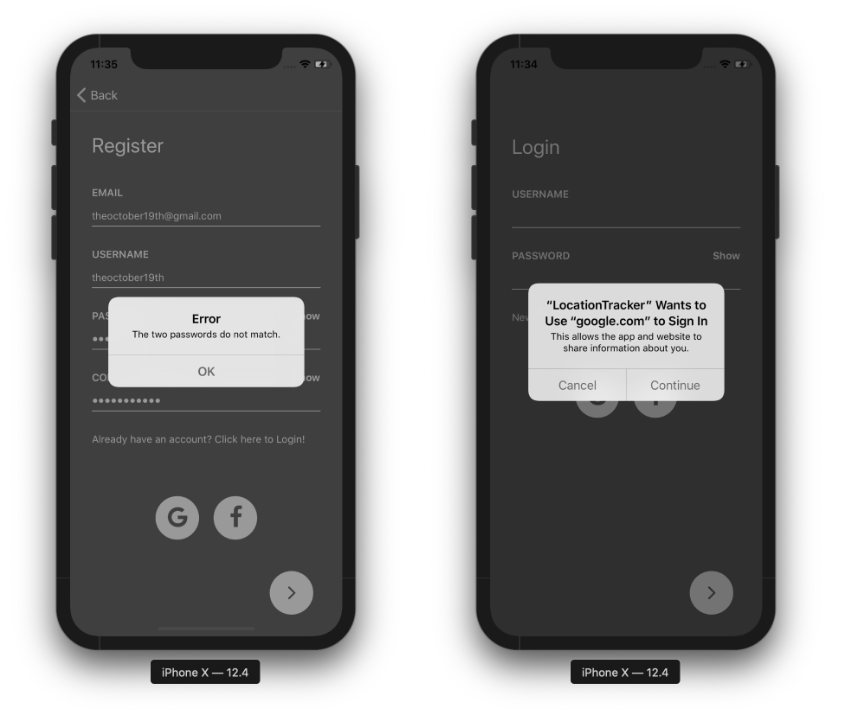
\includegraphics[width=\linewidth]{screenshots/2.png}	
\end{figure}



\begin{figure}[h]
\centering
	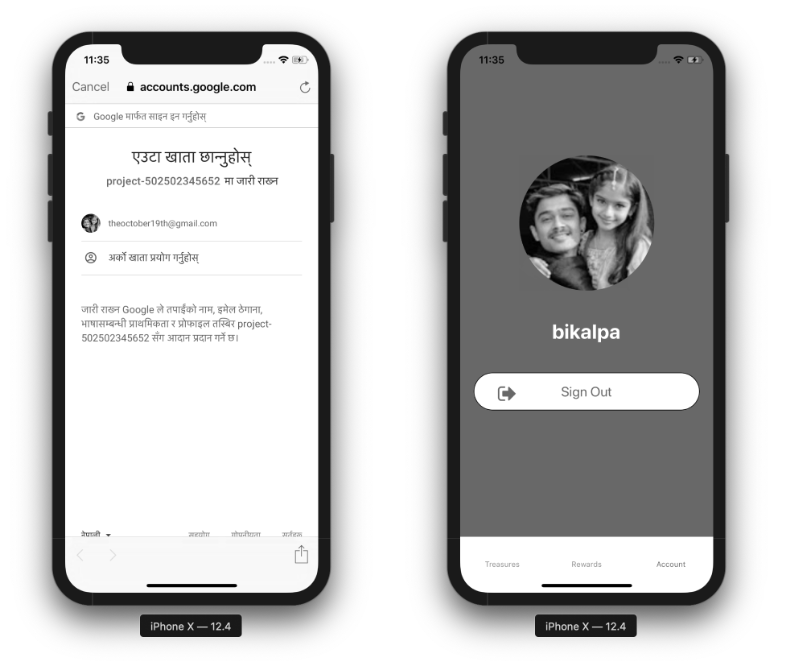
\includegraphics[width=\linewidth]{screenshots/3.png}
	\caption{Screenshots of the application developed}
	\label{fig:sc}	
\end{figure}



\pagebreak
\section{Results and Discussion}
At the point of submission of this document, the project is almost 65\% complete. The backend part is almost complete while some amount of task is remaining in application development part. After analysing the project schedule submitted earlier during proposal defense, our project is right on its proposed time schedule.

At this point in time, the project team has learnt a lot about the cross platform development and the basics of RESTful services as compared to when the project was just started. At first, the project team had used SQLite as the database due to its small size and easier integration and we later switched to the MySQL database. We had initially used SQLite only for test purpose. However during the migration of database we had to tackle a lot of portability issues and also required to re-enter the data to the database. We also had encountered problems while integrating third party authentication service (like Facebook and Google) to our project, partly because we were configuring our project to run both on Android and iOS devices simultaneously. However we were able to solve to the problem with team work and mutual discussion.

\pagebreak
\section{Tasks Remaining}
This section enlists the taks that are yet to be done before the final defense of the project.

\subsection{API Completion}
Although the authentication module is already working fine, we need to incorporate JWT (Java Web Token) model to authenticate every request to the backend API. Since we have already written logic for the generation of the key, the only thing remaining is to add a parameter called 'key' to every request, and then validate that key by API server before sending response to a client.

Similarly, the end points for the search queries have not yet been written. The API should be updated with provision of search queries for treasures as well as rewards. After completion of these two features, the backend API part of our project will be complete. On overall, about 80\% of work has been completed in the backend portion.

\subsection{Mobile Application Completion}
The mobile application part of the project has been completed to about 50\% of the total work required. Right now, the authentication module is working fine, which needs slight modifications for incorporating the JWT tokens mentioned earlier. The major work remaining in the application portion is to show treasure locations in the map and then write logic to collect those treasures when the user checks in using their app at that location.

\pagebreak
\section{ Deliverables}
The following will be the major deliverables that will be produced at the end of this project.

\subsection{RESTful API service}
There will be a running instance of RESTful API service developed and deployed at the end of the project. This API will be responsible for communicating between the client applications and the central database server.

\subsection{Android client application}
The application will be developed integrating all the features proposed earlier. The users will be able to use the application to scan QR codes at different travel destinations which will reward them with scores in their accounts. An interactive map will be integrated with the application that shows the treasures installed at various tourist destinations near to the tourist's current location. The application will also be integrated with social networking platforms like Facebook, Twitter, Instagram etc. so the tourists can share their scores publicly to their friends and acquaintances. 

\break
\section{Project Task and Time Schedule}
The working time period for the project is three months. The project will be completed by the end of the spring semester as per the requirements of the university. The major task division among the team members is mentioned in Table \ref{table:taskdiv}.

\begin{table}[h!]
\begin{tabular}{|l|l|}
\hline
\rowcolor[HTML]{C0C0C0} 
\textbf{Team Member} & \textbf{Assigned Tasks}                                                                                                                     \\ \hline
Bikalpa Dhakal       & \begin{tabular}[c]{@{}l@{}} Project Management\\Android Application Development\\ Deployment \end{tabular} \\ \hline
Avinash Shreshtha   & \begin{tabular}[c]{@{}l@{}}API Development\\ Data Management\\ Project Documentation\end{tabular}                                           \\ \hline
\end{tabular}
\caption{Division of tasks among project team members}
\label{table:taskdiv}
\end{table}

The time schedule of the project is illustrated in Figure \ref{fig:schedule}.

\begin{figure}[h!]
	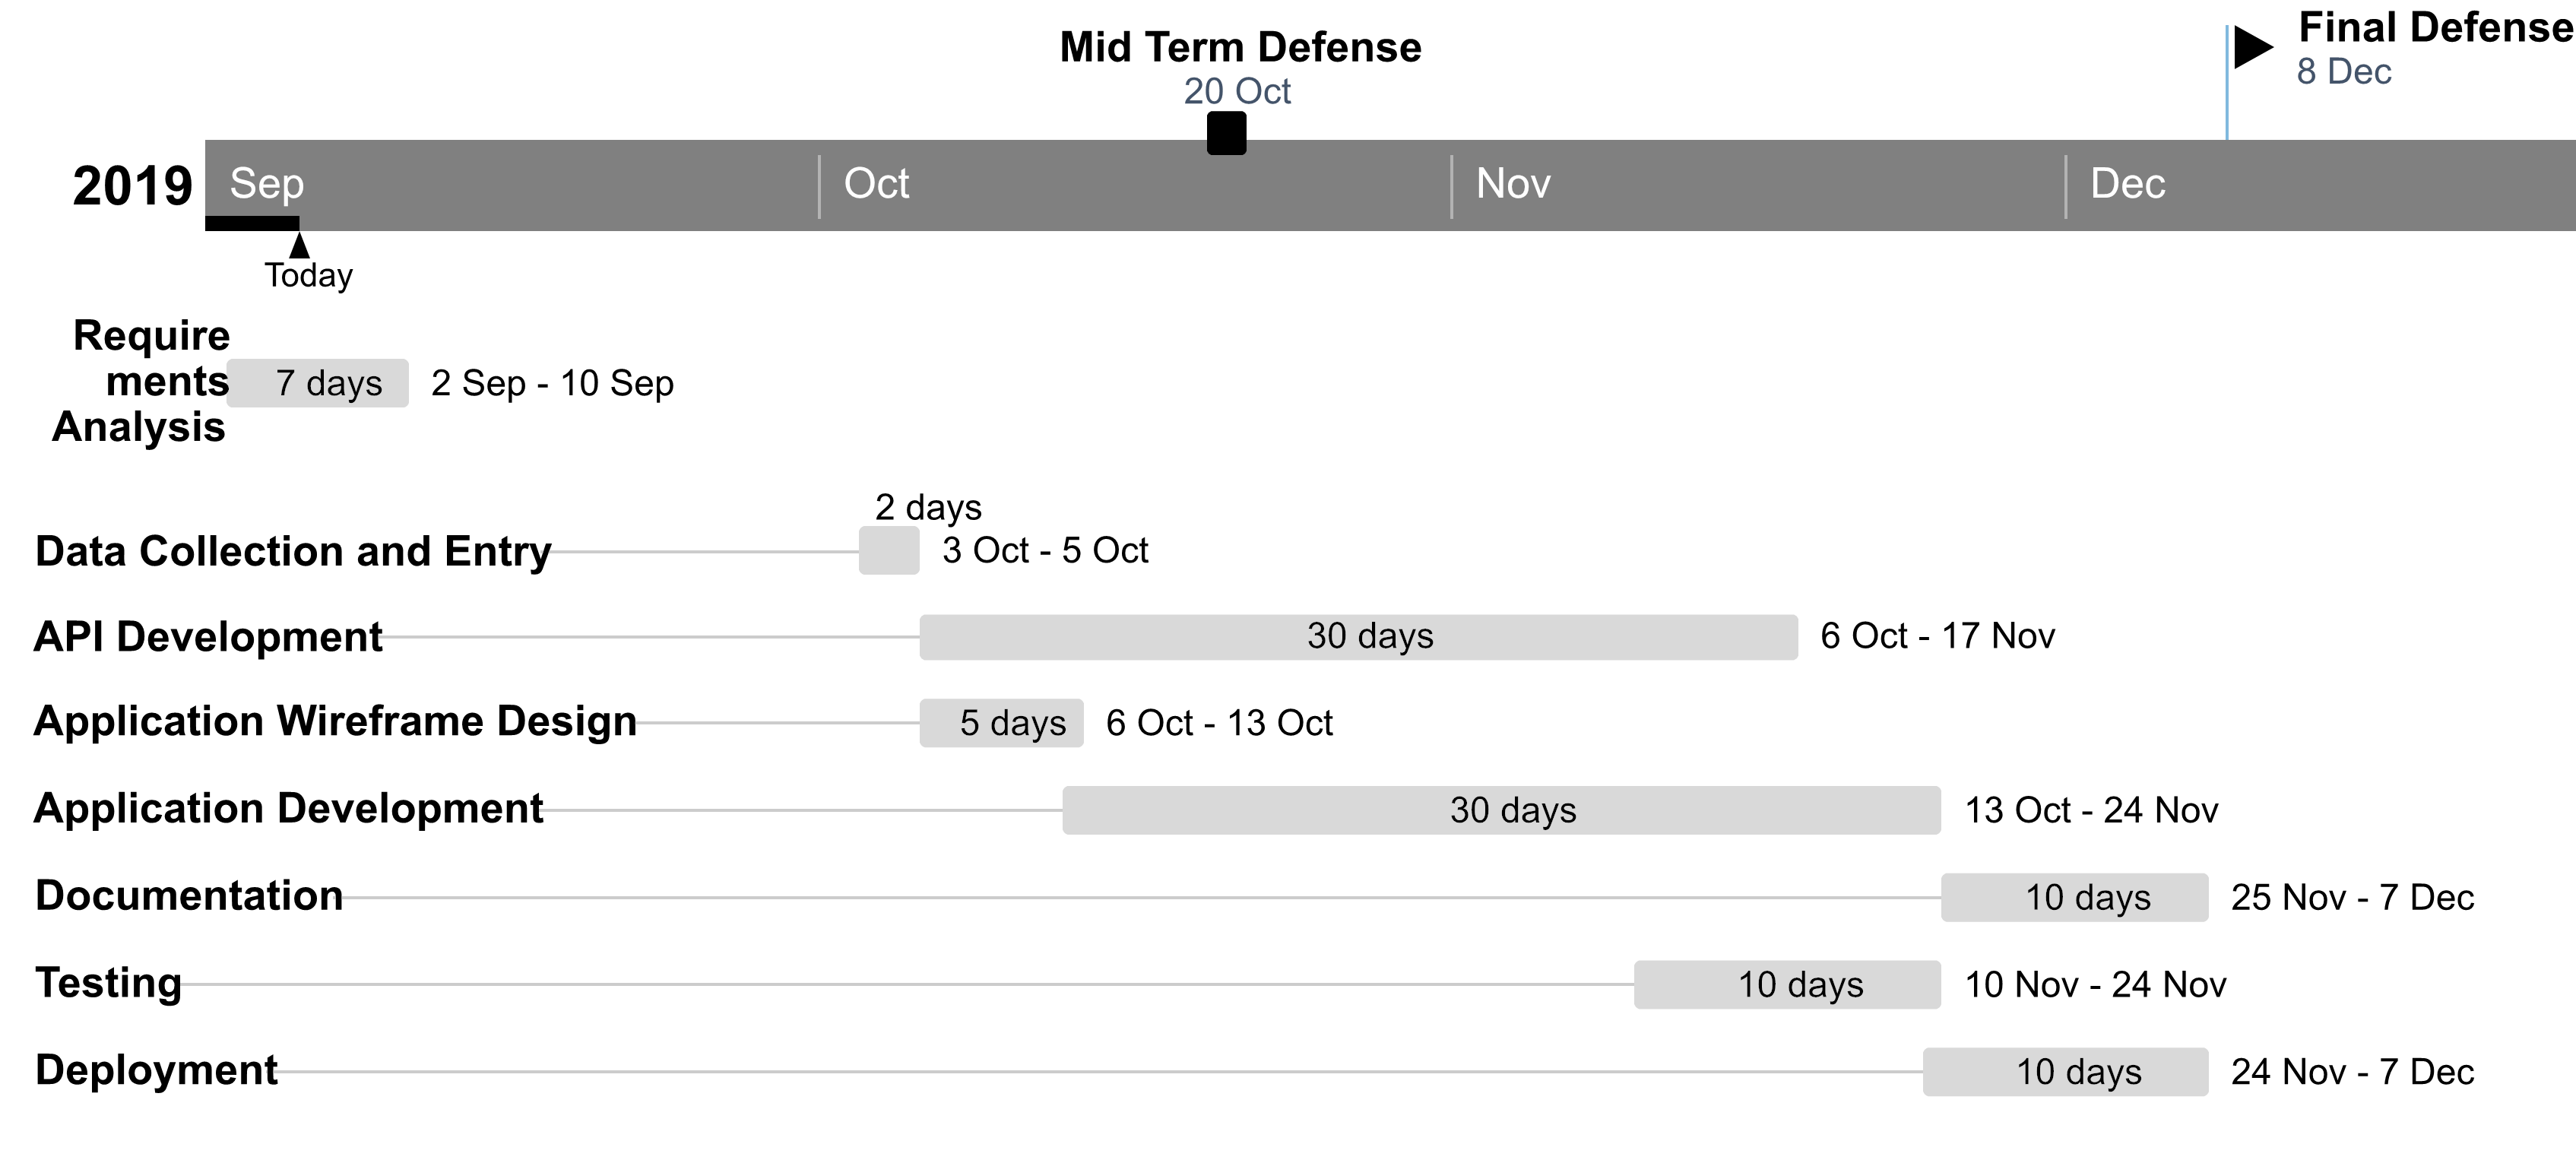
\includegraphics[width=\linewidth]{schedule}
	\centering
	\caption{Proposed project schedule}
	\label{fig:schedule}
\end{figure}



\break
\addcontentsline{toc}{section}{References}
\bibliography{references}
\bibliographystyle{ieeetran}

\end{document}

%\break
%\section{Proposed Performance Analysis Methodology}
%The performance analysis of the deliverables will be performed according to the popular Top Down Methodology. The main idea in this method is to analyse and address the higher order performance issues at first, then follow the lead upto the lower levels of details if needed \cite{tdmethod}. This methodology is proposed to be followed because it largely reduces the time and cost of assessing the performance since not every modules and sections of the project need to be analyzed at a deeper level.
%
%The final evaluation of the project will be performed by the project evaluation team designated by the college administration.
